\appendix

\section{Implementation Details}
\label{sec:implementation_details}
\textbf{Training Hyperparamters.} \method \ extends LW-DETR \citep{chen2024lw} for Neural Architecture Search. We highlight key differences in our training procedure below. First, we pseudo-label Objects-365 \citep{objects365} with SAM2 \citep{ravi2024sam2} to allow us to pre-train the segmentation and detection heads on the same data. We use a learning rate of 1e-4 (LW-DETR uses 4e-4), and a batch size of 128 (LW-DETR uses the same). Similar to DINOv3 \citep{simeoni2025dinov3}, we use an EMA scheduler since this is necessary for EMA to function. However, unlike DINOv3, we omit learning-rate warm-up. We clip all gradients greater than 0.1 and apply a per-layer multiplicative decay of 0.8 to preserve information (especially the earlier layers) in the DINOv2 backbone. We place our window attention blocks between layers \{0, 1, 3, 4, 6, 7, 9, 10\}, while LW-DETR places their window attention blocks between layers \{0, 1, 3, 6, 7, 9\}. Although we have the same number of windows, contiguous windowed blocks don't require an additional reshape operation, making our implementation slightly more efficient. Further, we train with more multi-scale resolutions (0.5 to 1.5 scale) than LW-DETR (0.7 to 1.4 scale) to ensure that the augmentation is symmetric around the default scale. Notably, we add resolution as a ``tunable knob'' in our NAS search space, while LW-DETR uses it as a form of data augmentation. Our model training and inference code is available on \href{https://github.com/roboflow/rf-detr}{GitHub}.

\textbf{Latency Evaluation.} We ensure fair evaluation between models by measuring detection accuracy and latency using the same artifact. To further standardize inference, we employ CUDA graphs in TensorRT, which pre-queue all kernels rather than requiring the CPU to launch them serially during execution. This optimization can accelerate some networks depending on the number and type of kernels used by the model. We observe that RT-DETR, LW-DETR, and \method \ benefit from this optimization. Further, CUDA graphs place LW-DETR on the same latency-accuracy curve as D-FINE, since CUDA graphs speed up LW-DETR but do not benefit D-FINE. We release our stand-alone latency benchmarking tool on \href{https://github.com/roboflow/single_artifact_benchmarking}{GitHub}.

\textbf{Pareto-Optimal Model Configurations in COCO.} We present the Pareto-Optimal \method \ and \method-Seg configurations in Tables \ref{tab:coco_det_config} and \ref{tab:coco_seg_config}. We highlight notable trends about \method's Pareto-Optimal architectures in Appendix \ref{appendix:trends}.

{
\setlength{\tabcolsep}{1.0em}
\begin{table}[h]
\caption{\textbf{\method \ COCO Detection Model Config.}}
\label{tab:coco_det_config}
\scalebox{0.8}{
\begin{tabular}{|c|c|c|c|c|c|c|}
\hline
\rowcolor{gray!10}
\textbf{Model Size} & \textbf{Resolution} & \textbf{Patch Size} & \textbf{Windows} & \textbf{Decoder Layers} & \textbf{Queries} & \textbf{Backbone} \\ \hline
N         &          384           &          16           &       2           &          2               &          300        &          DINOv2-S            \\ \hline
S         &          512           &         16            &        2          &          3               &         300         &            DINOv2-S          \\ \hline
M         &          576           &          16           &          2        &           4              &        300          &          DINOv2-S            \\ \hline
L         &          704           &         16            &         2         &            4             &       300           &          DINOv2-S            \\ \hline
XL        &          700           &           20          &        1          &           5              &       300           &          DINOv2-B            \\ \hline
2XL       &            880         &           20          &         2         &            5             &         300         &          DINOv2-B            \\ \hline
Max       &         828            &         12            &       1           &            6             &          300        &          DINOv2-B            \\ \hline
\end{tabular}
}
\end{table}
}

{
\setlength{\tabcolsep}{1.0em}
\begin{table}[h]
\caption{\textbf{\method-Seg COCO Segmentation Model Config.}}
\label{tab:coco_seg_config}
\scalebox{0.8}{
\begin{tabular}{|c|c|c|c|c|c|c|}
\hline
\rowcolor{gray!10}
\textbf{Model Size} & \textbf{Resolution} & \textbf{Patch Size} & \textbf{Windows} & \textbf{Decoder Layers} & \textbf{Queries} & \textbf{Backbone} \\ \hline
N         &         312            &         12            &      1            &             4            &          100        &           DINOv2-S           \\ \hline
S         &          384           &         12            &         2         &               4          &          100        &          DINOv2-S            \\ \hline
M         &          432           &        12             &       2           &             5            &        200          &        DINOv2-S              \\ \hline
L         &        504             &          12           &       2           &                5         &           300       &            DINOv2-S          \\ \hline
XL        &          624           &         12            &         2         &               6          &        300          &         DINOv2-S             \\ \hline
2XL       &         768            &           12          &      2            &              6           &          300        &          DINOv2-S            \\ \hline
Max       &          890           &          10           &         1         &             6           &         300         &           DINOv2-S           \\ \hline
\end{tabular}
}
\end{table}
}

\textbf{Parameter Sampling Grid.} Lastly, we present our sampling grid for training and inference below. Importantly, we only drop decoder layers and queries during inference. We uniformly sample configurations during training and perform grid search over all configurations during inference to find Pareto-Optimal model configurations. RF-DETR’s total training time is roughly two to four times as long as a non-NAS baseline, depending on the target dataset. However, \method \ can generate all size configurations from this single training run, while other non-NAS baselines must be re-trained for each new model size. We evaluate 6,468 network configurations (11 resolutions * 7 patch sizes * 7 decoder layers * 3 windows * 4 query settings) during architecture search. We estimate that this search takes approximately 10,000 GPU Hours (200 T4 GPUs * 48 hours). 

\textbf{Training Configurations}
\begin{itemize}
    \item Image Resolutions: 320, 384, 448, 512, 576, 640, 704, 768, 832, 896, 960
    \item Patch Sizes: 8, 10, 12, 16, 20, 24, 32
    \item Number of Decoder Layers: 6
    \item Number of Windows: 1, 2, 4
    \item Number of Queries: 300
\end{itemize}


\textbf{Inference Configurations}
\begin{itemize}
    \item Image Resolutions: 320, 384, 448, 512, 576, 640, 704, 768, 832, 896, 960
    \item Patch Sizes: 8, 10, 12 ,14, 16, 20, 24, 32
    \item Number of Decoder Layers: 0, 1, 2, 3, 4, 5, 6
    \item Number of Windows: 1, 2, 4
    \item Number of Queries: 50, 100, 200, 300
\end{itemize}

\section{Ablation on Query Tokens and Decoder Layers}
\label{appendix:query_decoder}

\begin{figure}[h]
    \centering
    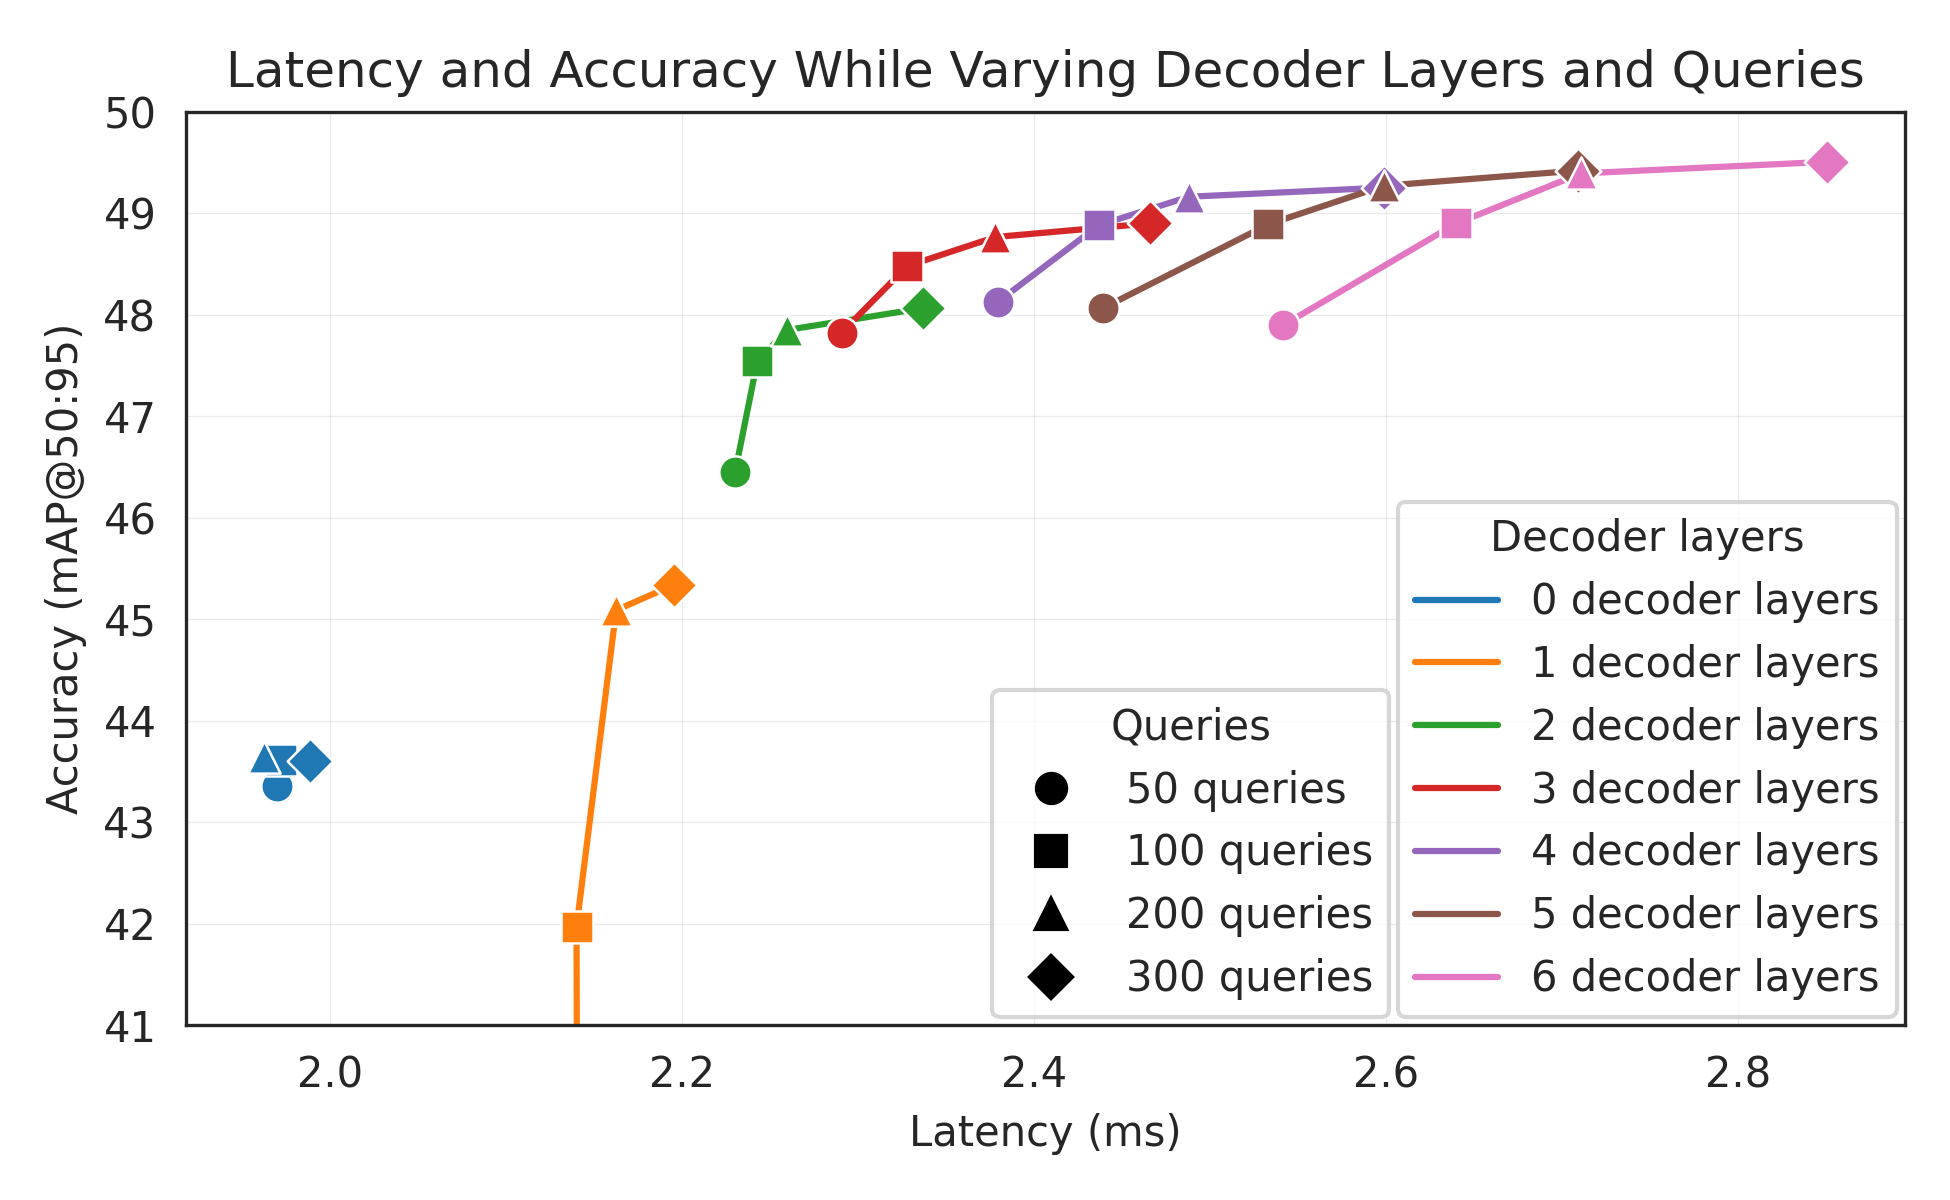
\includegraphics[width=0.98\linewidth]{figures/decoder_layers_queries_full.png}
    \caption{{\bf Impact of Decoder Layers vs. Query Tokens}. We evaluate the impact of inference-time query dropping for trading-off accuracy and latency in \method \ (nano). Interestingly, we find that dropping the 100 lowest confidence queries does not significantly reduce performance, but modestly improves latency for all decoder layers.}
    \label{fig:nas_query}
\end{figure}

We train \method \ (nano) with 300 object queries, following standard practices for real-time DETR-based object detectors. However, many datasets contain fewer than 300 objects per image. Therefore, processing all 300 queries can be computationally wasteful. LW-DETR (tiny) demonstrates that training with fewer queries can improve the latency-accuracy tradeoff. Rather than deciding on the optimal number of queries apriori, we find that we can drop queries at test time \textit{without retraining} by discarding the lowest-confidence queries ordered by the confidence of the corresponding token at the output of the encoder. As shown in Figure \ref{fig:nas_query}, this yields meaningful latency-accuracy tradeoffs. In addition, prior work \citep{zhao2024rtdetr} demonstrates that decoder layers can be pruned at test time, since each layer is supervised independently during training. We find that it is possible to remove \emph{all} decoder layers, relying solely on the initial query proposals from the two-stage DETR pipeline. In this case, there is no cross-attention to the encoder states or self-attention between queries, leading to a substantial runtime reduction. The resulting model resembles a single-stage YOLO-style architecture without NMS. Eliminating the final decoder layer reduces latency by 10\% with only a 2 mAP drop in performance.


\section{Benchmarking FLOPs}
We benchmark FLOPs for \method, GroundingDINO, and LLMDet with PyTorch's \href{https://github.com/pytorch/pytorch/blob/baee623691a38433d10843d5bb9bc0ef6a0feeef/torch/utils/flop_counter.py#L596}{\texttt{FlopCounterMode}}. We find that \texttt{FlopCounterMode} closely reproduces FLOP counts obtained with custom benchmarking tools for YOLOv11, D-FINE, and LW-DETR. In practice, we also find that it provides more reliable results than CalFLOPs \citep{calflops}. Notably, LW-DETR's FLOPs count is roughly twice that of the originally reported result (cf. Table \ref{tab:flops}). We posit that this discrepancy can be attributed to LW-DETR reporting MACs instead of FLOPs. We rely on the officially reported FLOPs counts from YOLOv11, YOLOv8, D-FINE, and RT-DETR.

{
\setlength{\tabcolsep}{3.4em}
\begin{table}[h]
\caption{\textbf{FLOPs Benchmarking Comparison.} We compare FLOPs reported with custom benchmarking tools, CalFLOPs, and PyTorch's FlopCounterMode. Notably, we find that FlopCounterModel closely matches the results reported with custom benchmarking code, suggesting that it is more reliable than prior generic benchmarking tools.}
\label{tab:flops}
\scalebox{0.7}{
\begin{tabular}{|lc|ccc|}\hline
\rowcolor{gray!10}
\hline
\textbf{Model} & \textbf{Size} & \textbf{Reported} & \textbf{CalFLOPs} & \textbf{FlopCounterMode} \\
\hline
D-FINE & S  & 25.2 M & 25.2 M & 25.5 M \\ \hline
LW-DETR & S & 16.6 M & 22.9 M & 31.8 M \\ \hline 
YOLO11 & S  & 21.5 M & 23.9 M & 21.6 M \\ \hline
\end{tabular}
}
\end{table}
}

\section{Impact of Class-Names on Open-Vocabulary Detectors}
We evaluate the impact of fine-tuning open-vocabulary detectors like GroundingDINO with class names on RF100-VL in Table \ref{tab:rf100-vl-class-names}. Intuitively, GroundingDINO's vision-language pre-training should be more more useful when we prompt with class names (e.g. {\tt car}, {\tt truck}, {\tt bus}) instead of class indices (e.g. 0, 1, 2). Using class names when fine-tuning provides more information to the VLM about the underlying data than is available to non-VLM detectors, potentially leading to better downstream performance. However, we find that fine-tuning GroundingDINO on RF100-VL yields nearly identical performance in both cases, suggesting that naively fine-tuning the end-to-end model mitigates the benefits of open-vocabulary pre-training. Future work should investigate ways of effectively fine-tuning VLMs to preserve foundational pre-training.

{
\setlength{\tabcolsep}{0.2em}
\begin{table}[h]
\caption{\textbf{Evaluating the Impact of Class Names.} We evaluate the impact of using class-names when fine-tuning VLMs like GroundingDINO. We find that class-names do not provide significant benefit over prompting with class indices, suggesting that fine-tuning has diminished the impact of internet-scale pre-training.
} 
\label{tab:rf100-vl-class-names}
\scalebox{0.7}{
\begin{tabular}{|lcccccccccc|}
\hline
\rowcolor{gray!10}
\textbf{Model} & \multicolumn{1}{c|}{\textbf{Size}} & \textbf{\# Params.} & \textbf{GFLOPS} & \multicolumn{1}{l|}{\textbf{Latency (ms)}} & \textbf{AP} & \textbf{AP$_{50}$} & \textbf{AP$_{75}$} & \textbf{AP$_S$} & \textbf{AP$_M$} & \textbf{AP$_L$} \\ \hline
%\rowcolor{gray!10}
%\multicolumn{11}{|l|}{\textbf{COCO}}                                                                \\ \hline
%\multicolumn{1}{|l|}{GroundingDINO \citep{liu2023grounding} w/ Standard Class Names}   & \multicolumn{1}{c|}{T}     &       &        & \multicolumn{1}{l|}{}             &    &      &      &     &     &     \\ \hline
%\multicolumn{1}{|l|}{GroundingDINO \citep{liu2023grounding} w/ Class Index Names}   & \multicolumn{1}{c|}{T}     &       &        & \multicolumn{1}{l|}{}             &    &      &      &     &     &     \\\hline
\rowcolor{gray!10}
\multicolumn{11}{|l|}{\textbf{RF100-VL}}                                                                \\ \hline
\multicolumn{1}{|l|}{GroundingDINO \citep{liu2023grounding} w/ Standard Class Names}   & \multicolumn{1}{c|}{T}     &   173.0M   &   1008.3     & \multicolumn{1}{c|}{309.9$^{*}$ }             &  62.3  &   88.8   &   67.8   &  39.2   &  57.7   &   69.5  \\ \hline
\multicolumn{1}{|l|}{GroundingDINO \citep{liu2023grounding} w/ Class Index Names}   & \multicolumn{1}{c|}{T}     &   173.0M   &   1008.3     & \multicolumn{1}{c|}{309.9$^{*}$ }             &  62.5  &   88.2   &   68.3   &  40.0   &   58.4  &  70.3   \\\hline
\end{tabular}
}
\end{table}
}

 
\section{Benchmarking Larger Model Variants}
\label{appendix:scaling}

Detectors like LW-DETR \citep{chen2024lw} and D-FINE \citep{peng2024dfine} hand-design larger variants to scale up a model family. In contrast, NAS-based architectures like \method \ automatically discover scaling strategies through grid-based search. We analyze two families of RF-DETR models derived from distinct scaling strategies: one based on a DINOv2-S backbone and another based on a DINOv2-B backbone. To evaluate how well each family scales, we compare their NAS-generated Pareto curves against those of D-FINE. Specifically, at each D-FINE size, we identify the RF-DETR variant with the same backbone that maximizes performance at a comparable latency. For example, when comparing to D-FINE (small), we select the RF-DETR model that offers the best accuracy without exceeding D-FINE (small)'s latency. Note that these \method models are different than those reported in Tables \ref{tab:coco_det} and \ref{tab:coco_det_scale}.

As shown in Table \ref{tab:scaling}, the DINOv2-S backbone family initially surpasses D-FINE in mAP@50:95 but fails to maintain this advantage at larger model sizes, suggesting that its scaling strategy is less effective than D-FINE's manual design. In contrast, the DINOv2-B backbone family shows the opposite trend, where the performance gap between D-FINE and \method \ narrows as latency increases. This implies that at higher latencies, the DINOv2-B based \method \ models could surpass D-FINE (and indeed RF-DETR (2x-large) outperforms D-FINE on mAP 50:95). Importantly, expanding the D-FINE model family would require substantial additional engineering effort, whereas extending the \method \ model family is straightforward; higher-latency variants can be sampled directly from the same NAS search without re-training. We present the COCO and RF100-VL results of our larger variants in Tables \ref{tab:coco_det_scale}, \ref{tab:coco_seg_scale}, and \ref{tab:rf100vl-scale}. We also include an \method \ Max variant on each dataset to show our method's maximum performance with latency less than 100ms, a scale other model families don't reach.

%When researchers build a new model family, they come up with a strategy as to how to give different members of the family different latency-accuracy tradeoffs. Looking at how accuracy increases with increasing compute gives a sense of how well that strategy scales. While families of hand-optimized models such as D-FINE require the manual curation of a strategy, NAS-based families can automatically discover their own scaling strategies within the constraints of the NAS search space. We consider two families of RF-DETR models generated by two different strategies, one from scaling a model based on a DINOv2-S backbone and the other from scaling based on a DINOv2-B backbone. To examine how well each model family scales, we consider the performance gap vs D-FINE of the NAS Pareto curve generated by each family at each of the D-FINE family's latencies. For D-FINE-S, for example, we consider the RF-DETR model with a given backbone that has the highest accuracy while still being faster than D-FINE-S. 

%The results of this experiment are available in Table \ref{tab:scaling}. We observe that, while the DINOv2-S backbone family initially outperforms D-FINE on mAP@50:95, the gap grows smaller and ultimately it underperforms D-FINE. From this perspective, the DINOv2-S family scales less well than the manually designed D-FINE scaling strategy. However, for DINOv2-B the opposite trend emerges: as we increase latency, the advantage of D-FINE over RF-DETR steadily decreases. Based on this, it is likely that at higher latencies the RF-DETR family based on DINOv2-B would begin to outperform D-FINE on mAP@50:95. However, because D-FINE is a family of hand-crafted models, generating additional models in the family would require significant additional work. For RF-DETR, on the other hand, we can simply take higher latency members of the same NAS search to extend the family, requiring no extra work beyond the initial training run. Note that for this example none of the RF-DETR models were trained beyond their initial NAS training.

{
\setlength{\tabcolsep}{3.7em}
\begin{table}[t]
\caption{\textbf{mAP@50:95 Gap of \method \ vs D-FINE at Similar Latencies} We compare how different \method \ model families scale relative to D-FINE. D-FINE (nano) is excluded since it was not pretrained on Objects-365 and is therefore not expected to follow similar scaling trends. For each \method \ backbone, we select the highest accuracy Pareto-optimal NAS-mined model with latency up to that of the corresponding D-FINE variant. Notably, \method \ (DINOv2-B) achieves better scalability than \method \ (DINOv2-S) and D-FINE. Note that none of the RF-DETR models for COCO are finetuned.}
\label{tab:scaling}
\scalebox{0.7}{
\begin{tabular}{|l|c|c|c|c|}\hline
\rowcolor{gray!10}
\hline
\textbf{Method (Backbone)}& \textbf{S} & \textbf{M} & \textbf{L} & \textbf{XL} \\
\hline
D-FINE  \citep{peng2024dfine}      & 50.6 & 55.4 & 57.2 & 59.3  \\ \hline
\method \ (DINOv2-S) & +2.3 & +0.9 & -0.4 & -1.1 \\ \hline 
\method \ (DINOv2-B) & -3.1 & -1.3 & -1.2 & -0.7 \\ \hline
\end{tabular}
}
\end{table}
}


{
\setlength{\tabcolsep}{0.65em}
\begin{table}[t]
\caption{\textbf{COCO Detection Evaluation for Larger Model Variants.} We present \method's performance for L, XL, and 2XL sizes on COCO below. Notably, D-FINE (x-large) outperforms \method \ (x-large) on mAP 50:95. However, \method \ (2x-large) beats D-FINE by 0.8 AP, and is the first real-time detector to surpass 60 AP on COCO.}
\label{tab:coco_det_scale}
\scalebox{0.7}{
\begin{tabular}{|lcccccccccc|}
\hline
\rowcolor{gray!10}
\textbf{Model} & \multicolumn{1}{c|}{\textbf{Size}} & \textbf{\# Params.} & \textbf{GFLOPS} & \multicolumn{1}{c|}{\textbf{Latency (ms)}} & \textbf{AP} & \textbf{AP$_{50}$} & \textbf{AP$_{75}$} & \textbf{AP$_S$} & \textbf{AP$_M$} & \textbf{AP$_L$} \\ \hline
\rowcolor{gray!10}
\multicolumn{11}{|l|}{\textbf{Real-Time Object Detection w/ NMS}}  \\ \hline
\multicolumn{1}{|l|}{YOLOv8 \citep{yolov8}}     & \multicolumn{1}{c|}{L}     &   43.7M    &    165.2    & \multicolumn{1}{c|}{8.0}             &   49.5   &   64.7   &  54.0    &   30.2   &   55.1   &   68.5   \\ \hline
\multicolumn{1}{|l|}{YOLOv11 \citep{yolov11}}     & \multicolumn{1}{c|}{L}     &   25.3M    &    86.9    & \multicolumn{1}{c|}{6.5}             &  49.9   &   64.9   &   54.5   &  30.4    &   55.9   &   68.1   \\ \hline \hline
\multicolumn{1}{|l|}{YOLOv8 \citep{yolov8}}     & \multicolumn{1}{c|}{XL}     &   68.2M    &     257.8   & \multicolumn{1}{c|}{11.3}             &  50.5   &   65.6   &   55.1   &   30.0   &   56.2   &   69.5   \\ \hline
\multicolumn{1}{|l|}{YOLOv11 \citep{yolov11}}     & \multicolumn{1}{c|}{XL}     &   56.9M    &    194.9    & \multicolumn{1}{c|}{10.5}             &   50.9  &  66.1    &   55.4   &   31.5   &   56.6   &   68.7   \\ \hline \hline
\rowcolor{gray!10}
\multicolumn{11}{|l|}{\textbf{End-to-End Real-Time Object Detection}}                                                                \\ \hline
\multicolumn{1}{|l|}{RT-DETR \citep{zhao2024rtdetr}}      & \multicolumn{1}{c|}{R50}     &   42M    &    136    & \multicolumn{1}{c|}{8.5}             &      55.0   &   73.3   &  59.8 & 37.9  &  59.7    &   71.6   \\ \hline
\multicolumn{1}{|l|}{LW-DETR \citep{chen2024lw}}      & \multicolumn{1}{c|}{L}     &   46.8M    &     137.5     & \multicolumn{1}{c|}{6.9}             &   56.1  &   74.6   &   61.0   &   37.1   &  60.4    &   73.0   \\ \hline
\multicolumn{1}{|l|}{D-FINE \citep{peng2024dfine}}      & \multicolumn{1}{c|}{L}     &    31M   &    91    & \multicolumn{1}{c|}{7.5}             &  57.2   &   74.9   &   62.2   &   40.6   &    61.4  &   73.7   \\ \hline
\multicolumn{1}{|l|}{\method \ (Ours)}     & \multicolumn{1}{c|}{L}     &   33.9M    &    125.6    & \multicolumn{1}{c|}{6.8}             &   56.5  &  75.1    &   61.3   &   39.0   &  61.0    &   73.9   \\ \hline \hline
%\multicolumn{1}{|l|}{\method \ (Ours) w/ Fine-Tuning}     & \multicolumn{1}{c|}{L}     &    33.9M   &   125.6     & \multicolumn{1}{c|}{6.8}             &   56.5  &   75.1   &   61.3   &   38.9   &   61.1   &  74.0    \\ \hline \hline
\multicolumn{1}{|l|}{RT-DETR \citep{zhao2024rtdetr}}      & \multicolumn{1}{c|}{R101}     &   76M    &    259    & \multicolumn{1}{c|}{12.0}             &   56.1  &   74.5   &   61.1   &   38.1   &   60.4   &   73.4   \\ \hline
\multicolumn{1}{|l|}{LW-DETR \citep{chen2024lw}}      & \multicolumn{1}{c|}{XL}     &    118.0M   &   342.5      & \multicolumn{1}{c|}{13.0}             &  58.3   &  76.9    &   63.3   &   40.2   &  63.3    &   74.7   \\ \hline
\multicolumn{1}{|l|}{D-FINE \citep{peng2024dfine}}      & \multicolumn{1}{c|}{XL}     &   62M    &    202    & \multicolumn{1}{c|}{11.5}             &  59.3   &   76.8   &   64.6   &  42.1    &  64.2    &   76.3   \\ \hline
\multicolumn{1}{|l|}{\method \ (Ours)}     & \multicolumn{1}{c|}{XL}     &   126.4M    &    299.3    & \multicolumn{1}{c|}{11.5}             &   58.6  &    77.4  &   63.8   &   40.3   &  63.9    &   76.2   \\ \hline \hline
%\multicolumn{1}{|l|}{\method \ (Ours) w/ Fine-Tuning}     & \multicolumn{1}{c|}{XL}     &    126.4M   &   299.3     & \multicolumn{1}{c|}{11.5}             &  58.9   &  77.5    &   64.0   &   40.8   &   64.3   &   76.3   \\ \hline \hline
\multicolumn{1}{|l|}{\method \ (Ours)}     & \multicolumn{1}{c|}{2XL}     &    126.9M   &    438.4    & \multicolumn{1}{c|}{17.2}             &  60.1   &   78.5   &   65.5   &   43.2   &   64.9   &   76.2   \\ \hline \hline
%\multicolumn{1}{|l|}{\method \ (Ours) w/ Fine-Tuning}     & \multicolumn{1}{c|}{2XL}     &    126.9M   &   438.4     & \multicolumn{1}{c|}{17.2}             &  60.2   &   78.5   &   65.8   &   43.7   &   65.1   &   76.3   \\ \hline \hline
\multicolumn{1}{|l|}{\method \ (Ours)}     & \multicolumn{1}{c|}{Max}     &   132.4M    &    1742.5    & \multicolumn{1}{c|}{98.0}             &  61.8   &   79.7   &   67.7   &  47.5    &   66.1   &   76.0   \\ \hline
\end{tabular}
}
\end{table}
}


{
\setlength{\tabcolsep}{0.65em}
\begin{table}[t]
\caption{\textbf{COCO Segmentation Evaluation for Larger Model Variants.} We present \method's performance for L, XL, and 2XL sizes on the COCO segmentation benchmark below. We find that scaling up \method \ yields considerable performance improvements. In contrast, YOLOv8 and YOLOv11 do not significantly improve with scale.}
\label{tab:coco_seg_scale}
\scalebox{0.7}{
\begin{tabular}{|lcccccccccc|}
\hline
\rowcolor{gray!10}
\textbf{Model} & \multicolumn{1}{c|}{\textbf{Size}} & \textbf{\# Params.} & \textbf{GFLOPS} & \multicolumn{1}{c|}{\textbf{Latency (ms)}} & \textbf{AP} & \textbf{AP$_{50}$} & \textbf{AP$_{75}$} & \textbf{AP$_S$} & \textbf{AP$_M$} & \textbf{AP$_L$} \\ \hline
\rowcolor{gray!10}
\multicolumn{11}{|l|}{\textbf{Real-Time Instance Segmentation w/ NMS}}  \\ \hline
\multicolumn{1}{|l|}{YOLOv8 \citep{yolov8}}     & \multicolumn{1}{c|}{L}     &   46.0M    &    220.5    & \multicolumn{1}{c|}{9.7}             &  39.0   &   60.5   &   41.7   &   18.0   &   44.7   &   57.8   \\ \hline
\multicolumn{1}{|l|}{YOLOv11 \citep{yolov11}}     & \multicolumn{1}{c|}{L}     &   27.6M    &    132.2    & \multicolumn{1}{c|}{8.3}             &  39.5   &   61.5   &  42.1    &  18.6    &   45.5   &   59.4   \\ \hline \hline
\multicolumn{1}{|l|}{YOLOv8 \citep{yolov8}}     & \multicolumn{1}{c|}{XL}     &   71.8M    &    344.1    & \multicolumn{1}{c|}{14.0}             &  39.5   &   61.3   &   42.1   &   18.9   &   45.6   &   58.8   \\ \hline
\multicolumn{1}{|l|}{YOLOv11 \citep{yolov11}}     & \multicolumn{1}{c|}{XL}     &    62.1M   &     296.4   & \multicolumn{1}{c|}{13.7}             &   40.1  &   62.4   &  42.6    &   18.8   &   46.4   &   60.1   \\ \hline \hline
\rowcolor{gray!10}
\multicolumn{11}{|l|}{\textbf{End-to-End Real-Time Instance Segmentation}}                                                                \\ \hline
\multicolumn{1}{|l|}{\method \ (Ours)}     & \multicolumn{1}{c|}{L}     &    36.2M   &   151.1     & \multicolumn{1}{c|}{8.8}             &   47.1  &   70.5   &   50.9   &   28.4   &  52.1    &   65.6   \\ \hline
%\multicolumn{1}{|l|}{\method \ (Ours) w/ Fine-Tuning}     & \multicolumn{1}{c|}{L}     &       &        & \multicolumn{1}{c|}{}             &     &      &      &      &      &      \\ \hline \hline
\multicolumn{1}{|l|}{\method \ (Ours)}     & \multicolumn{1}{c|}{XL}     &    38.1M   &    260.0    & \multicolumn{1}{c|}{13.5}             &  48.8   &   72.2   &   53.1   &   30.6   &   53.3   &   65.9    \\ \hline
%\multicolumn{1}{|l|}{\method \ (Ours) w/ Fine-Tuning}     & \multicolumn{1}{c|}{XL}     &       &        & \multicolumn{1}{c|}{}             &     &      &      &      &      &      \\ \hline \hline
\multicolumn{1}{|l|}{\method \ (Ours)}     & \multicolumn{1}{c|}{2XL}     &   38.6M    &    435.3    & \multicolumn{1}{c|}{21.8}             &   49.9  &   73.1   &   54.5   &   33.9   &   54.1   &   65.7   \\ \hline
%\multicolumn{1}{|l|}{\method \ (Ours) w/ Fine-Tuning}     & \multicolumn{1}{c|}{2XL}     &       &        & \multicolumn{1}{c|}{}             &     &      &      &      &      &      \\ \hline \hline
\multicolumn{1}{|l|}{\method \ (Ours)}     & \multicolumn{1}{c|}{Max}     &    40.1M   &    1668.2    & \multicolumn{1}{c|}{95.6}             &  50.5   &   74.0   &   55.4   &   34.6   &   54.2   &   65.4   \\ \hline
\end{tabular}
}
\end{table}
}


{
\setlength{\tabcolsep}{0.65em}
\begin{table}[t]
\caption{\textbf{RF100-VL Detection Evaluation for Larger Model Variants.} We present \method's performance for L, XL, and 2XL sizes on RF100-VL below. Notably, \method \ (x-large) beats D-FINE by 0.5 AP. Fine-tuning \method \ (x-large) improves performance by an additional 0.4 AP.}
\label{tab:rf100vl-scale}
\scalebox{0.7}{
\begin{tabular}{|lcccccccccc|}
\hline
\rowcolor{gray!10}
\textbf{Model} & \multicolumn{1}{c|}{\textbf{Size}} & \textbf{\# Params.} & \textbf{GFLOPS} & \multicolumn{1}{c|}{\textbf{Latency (ms)}} & \textbf{AP} & \textbf{AP$_{50}$} & \textbf{AP$_{75}$} & \textbf{AP$_S$} & \textbf{AP$_M$} & \textbf{AP$_L$} \\ \hline
\rowcolor{gray!10}
\multicolumn{11}{|l|}{\textbf{Real-Time Object Detection w/ NMS}}  \\ \hline
\multicolumn{1}{|l|}{YOLOv8 \citep{yolov8}}     & \multicolumn{1}{c|}{L}     &   43.7M    &    165.2     & \multicolumn{1}{c|}{7.9}             &  56.5   &  82.1    &   61.1   &   7.1   &   46.0   &    48.9  \\ \hline
\multicolumn{1}{|l|}{YOLOv11 \citep{yolov11}}     & \multicolumn{1}{c|}{L}    &   25.3M    &    86.9      & \multicolumn{1}{c|}{6.4}             &  56.5   &  82.2    &  61.0    &  6.4    &   45.5   &   49.0   \\ \hline \hline
\multicolumn{1}{|l|}{YOLOv8 \citep{yolov8}}     & \multicolumn{1}{c|}{XL}   &   68.2M    &     257.8      & \multicolumn{1}{c|}{11.2}             &  56.5   &  82.3    &  61.0    &   6.6   &   45.7   &   47.9   \\ \hline
\multicolumn{1}{|l|}{YOLOv11 \citep{yolov11}}     & \multicolumn{1}{c|}{XL}   &   56.9M    &    194.9      & \multicolumn{1}{c|}{10.3}             &  56.2   &   81.7   &   60.8   &  6.1    &   45.9   &   48.1   \\ \hline \hline
\rowcolor{gray!10}
\multicolumn{11}{|l|}{\textbf{End-to-End Real-Time Object Detection}}                                                                \\ \hline
\multicolumn{1}{|l|}{RT-DETR \citep{zhao2024rtdetr}}      & \multicolumn{1}{c|}{R50}     &   42M    &    136    & \multicolumn{1}{c|}{8.4}             &  61.7   &   87.7   &  66.9    &   38.1   &   57.1   &  69.4    \\ \hline
\multicolumn{1}{|l|}{LW-DETR \citep{chen2024lw}}      & \multicolumn{1}{c|}{L}     &   46.8M    &     137.5   & \multicolumn{1}{c|}{6.8}             &  61.5   &   87.4   &   67.0   &   37.1   &  56.4    &   69.0   \\ \hline
\multicolumn{1}{|l|}{D-FINE \citep{peng2024dfine}}      & \multicolumn{1}{c|}{L}     &     31M   &    91   & \multicolumn{1}{c|}{7.5}             & 61.6    &  86.4    &  67.2    &  37.8    &  56.5    &   70.1   \\ \hline
\multicolumn{1}{|l|}{\method \ (Ours)}     & \multicolumn{1}{c|}{L}     &   34.1M    &    119.1    & \multicolumn{1}{c|}{6.2}             &  62.0   &   88.1   &   67.3   &  36.9    &   57.1   &   70.2   \\ \hline
\multicolumn{1}{|l|}{\method \ (Ours) w/ Fine-Tuning}     & \multicolumn{1}{c|}{L}     &   34.1M    &    119.1     & \multicolumn{1}{c|}{6.2}             &  62.3   &   88.2   &   67.4   &   37.1   &   57.2   &  70.3    \\ \hline \hline
\multicolumn{1}{|l|}{RT-DETR \citep{zhao2024rtdetr}}      & \multicolumn{1}{c|}{R101}     &   76M    &    259   & \multicolumn{1}{c|}{11.9}             &  61.0   &  87.4    &  66.2    &  36.6    &  56.3    &  68.2    \\ \hline
\multicolumn{1}{|l|}{LW-DETR \citep{chen2024lw}}      & \multicolumn{1}{c|}{XL}     &    118.0M   &   342.5     & \multicolumn{1}{c|}{13.0}             &  62.1   &  87.9    &  67.6    &  37.4    &  57.1    &   70.2   \\ \hline
\multicolumn{1}{|l|}{D-FINE \citep{peng2024dfine}}      & \multicolumn{1}{c|}{XL}     &    59.3   &   76.8     & \multicolumn{1}{c|}{11.4}             &  62.2   &  86.9    &   68.0   &  37.6    &   57.4   &   69.7   \\ \hline
\multicolumn{1}{|l|}{\method \ (Ours)}     & \multicolumn{1}{c|}{XL}     &   35.0M    &    199.0    & \multicolumn{1}{c|}{9.7}             &   62.6   &  88.5   &  67.9   &   39.0   &   57.8   &  70.4  \\ \hline
\multicolumn{1}{|l|}{\method \ (Ours) w/ Fine-Tuning}     & \multicolumn{1}{c|}{XL}     &  35.0M    &    199.0      & \multicolumn{1}{c|}{9.7}             &   63.0  &   88.7   &   68.2   &   38.8   &   58.2   &   70.6   \\ \hline \hline
\multicolumn{1}{|l|}{\method \ (Ours)}     & \multicolumn{1}{c|}{2XL}     &   123.5M    &    410.2   & \multicolumn{1}{c|}{15.6}             &  63.3   &   88.9   &    69.0  &  38.7    &   58.2   &   71.6   \\ \hline
\multicolumn{1}{|l|}{\method \ (Ours) w/ Fine-Tuning}     & \multicolumn{1}{c|}{2XL}     &   123.5M    &    410.2    & \multicolumn{1}{c|}{15.6}             &   63.5  &   89.0   &   69.2   &   38.9   &   58.3   &   71.7   \\ \hline
\end{tabular}
}
\end{table}
}

\section{Per-Knob Sensitivity Analysis}
\label{appendix:tunable-knobs}

We evaluate the impact of varying resolution and patch size in Figure \ref{fig:knob_sensitivity}. Both curves follow a clear Pareto frontier, and are consistent with findings from prior work like FlexiViT \citep{beyer2023flexivit}. \method \ is able to gracefully interpolate between seen (blue circles) and unseen (red stars) configurations during inference. Importantly, unseen configurations closely track the trend established by the seen configurations, demonstrating that RF-DETR generalizes beyond the model configurations encountered during training. 

\begin{figure}
    \centering
    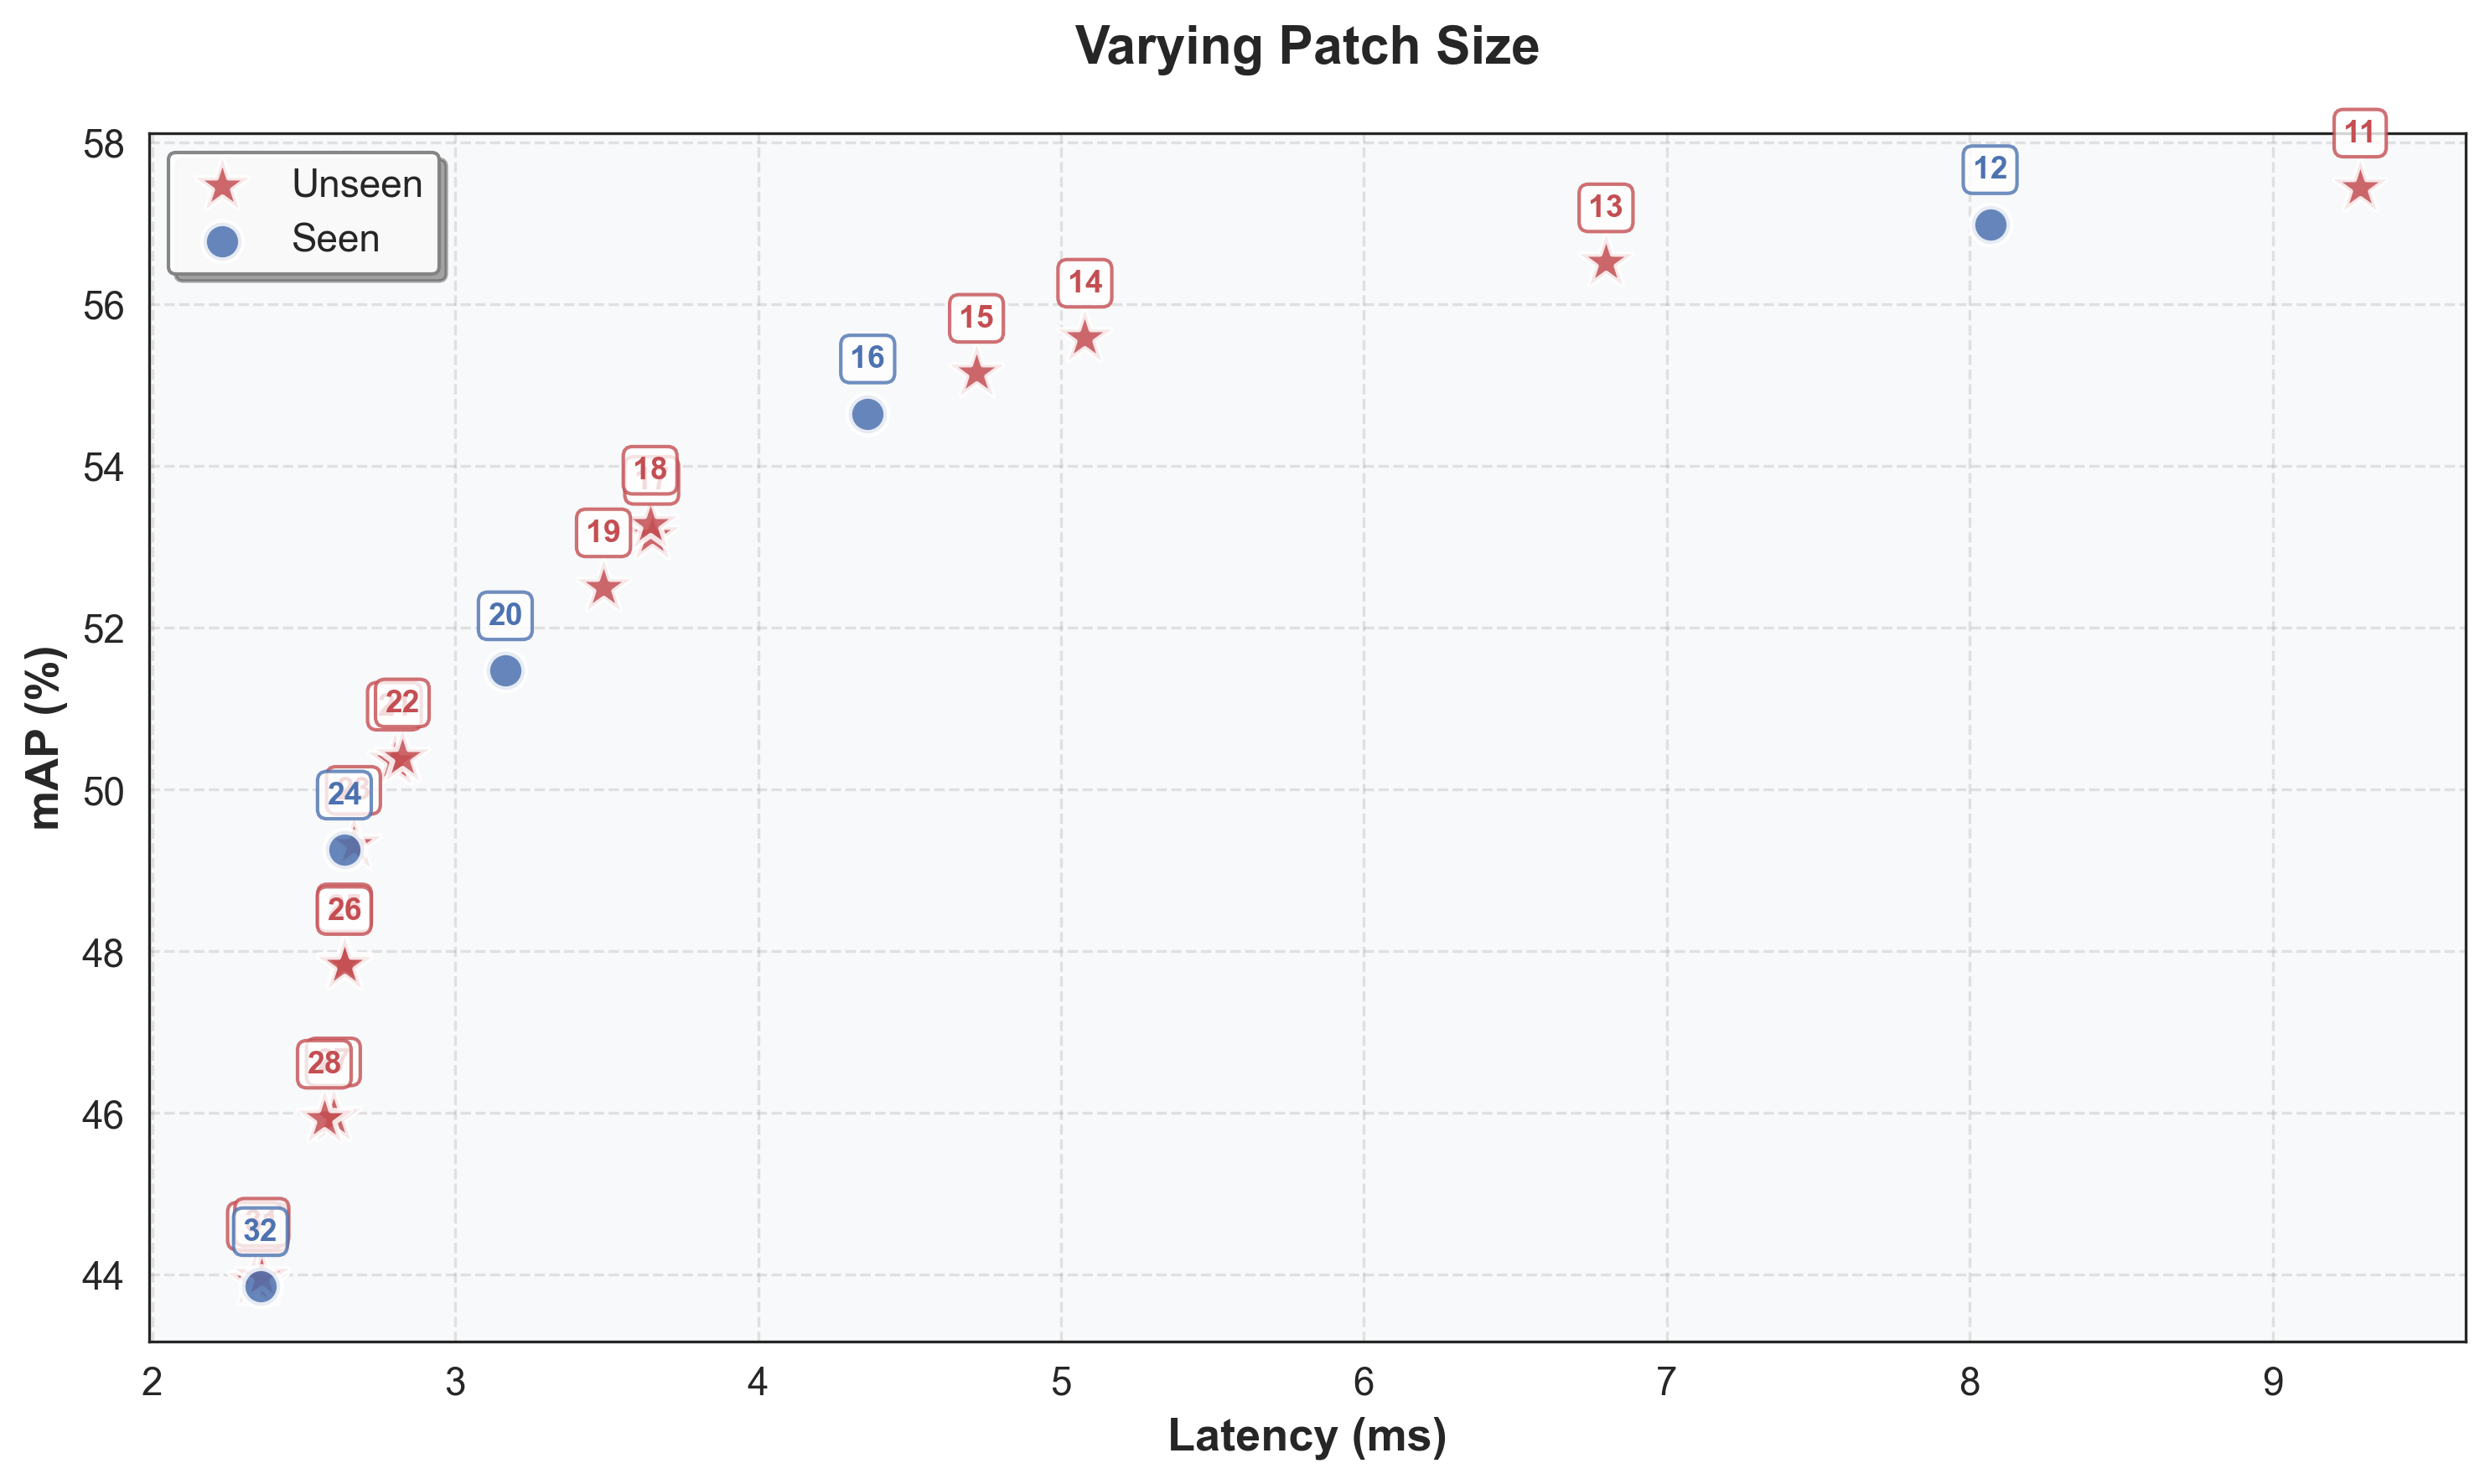
\includegraphics[width=0.48\linewidth]{figures/knob_turning_patch_size.png}
    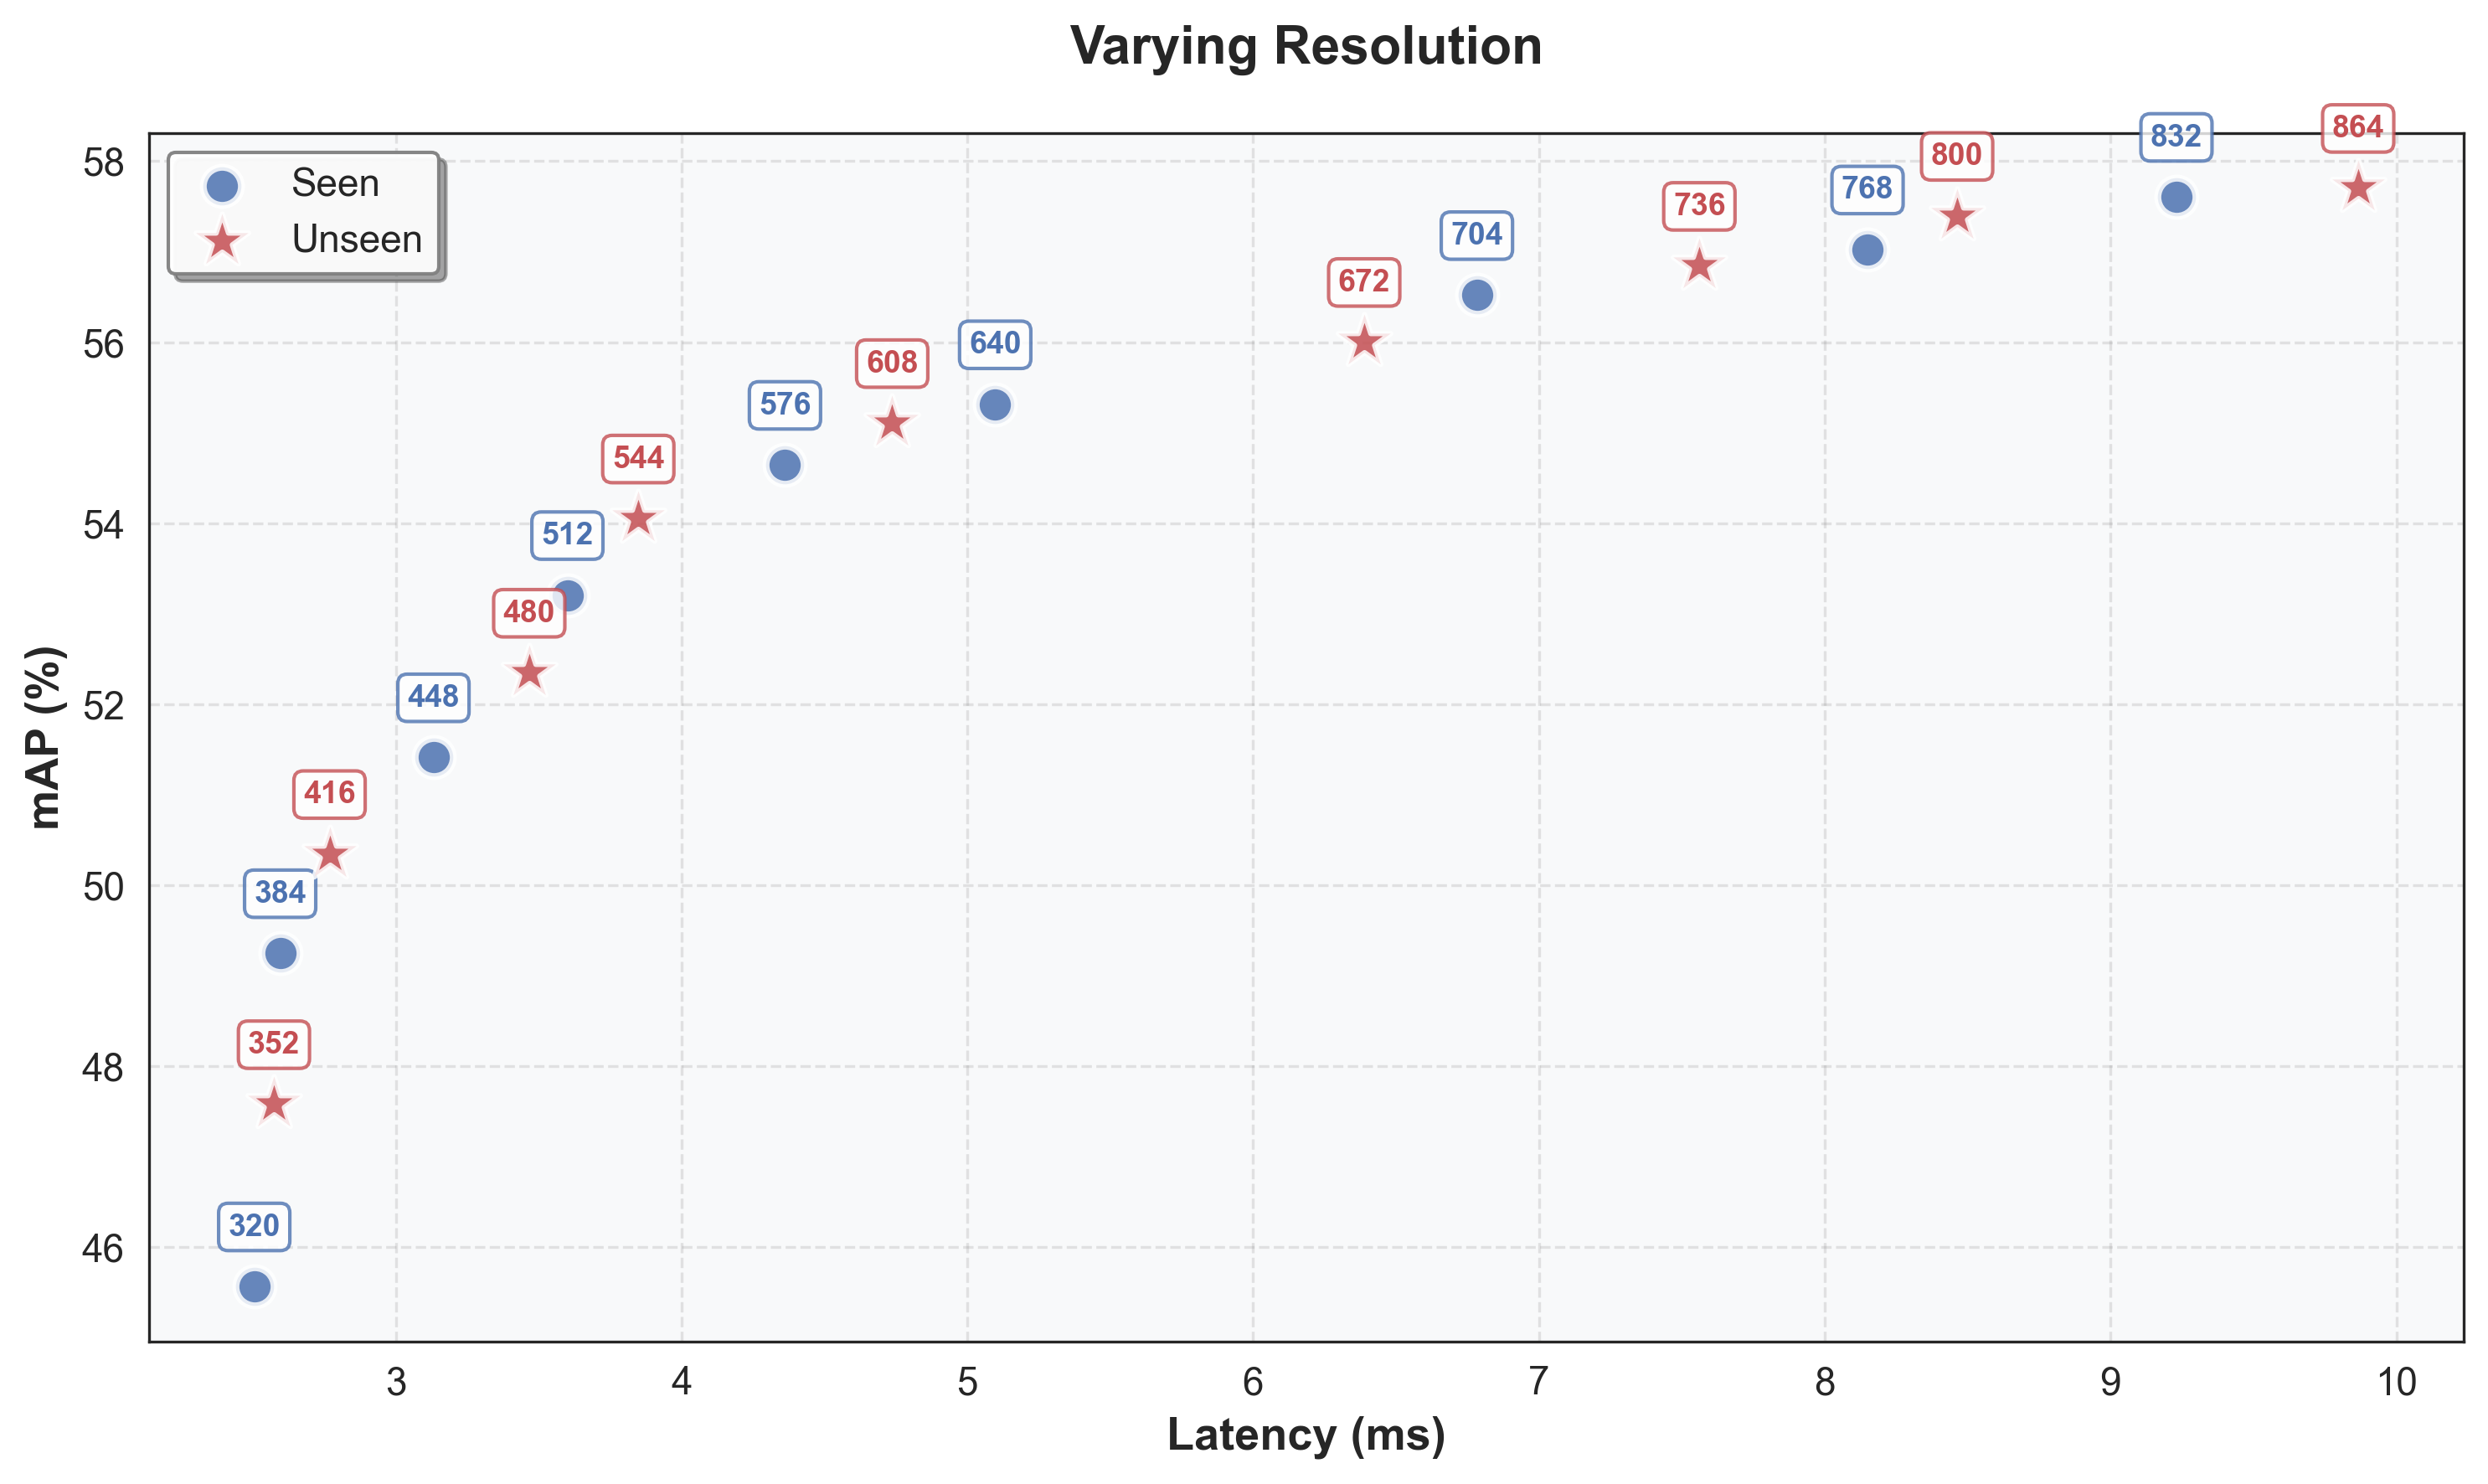
\includegraphics[width=0.48\linewidth]{figures/knob_turning_resolution.png}
    \caption{\textbf{Per Knob Sensitivity Analysis.} Despite never seeing certain resolutions and patch sizes, \method \ is able to gracefully interpolate to novel model configurations. }
    \label{fig:knob_sensitivity}
\end{figure}

\section{Impact of NAS Fine-Tuning on COCO}
\label{appendix:fine-tuning}
We find that fine-tuning after NAS provides limited benefit for COCO. We posit that the NAS ``architecture augmentation'' acts as a strong regularizer, and additional training without this regularization leads to degraded performance. Specifically, when models are pre-trained with strong regularization, removing the regularization during fine-tuning leads to overfitting. As shown in Tables \ref{tab:coco-det-ft} and \ref{tab:coco-seg-ft}, this trend is consistent across both detection and segmentation tasks. Interestingly, models trained on RF100-VL benefit more from fine-tuning, likely because they require more than 100 epochs to converge. In such cases, we posit that reducing the total number of NAS configurations during training, or training for more than 100 epochs with weight-sharing NAS can improve performance. 

{
\setlength{\tabcolsep}{0.65em}
\begin{table}[h]
\caption{\textbf{COCO Detection Fine-Tuning Evaluation.} We find that fine-tuning after NAS provides limited benefit for COCO detection, particularly for larger model sizes.} 
\label{tab:coco-det-ft}
\scalebox{0.7}{
\begin{tabular}{|lcccccccccc|}
\hline
\rowcolor{gray!10}
\textbf{Model} & \multicolumn{1}{c|}{\textbf{Size}} & \textbf{\# Params.} & \textbf{GFLOPS} & \multicolumn{1}{l|}{\textbf{Latency (ms)}} & \textbf{AP} & \textbf{AP$_{50}$} & \textbf{AP$_{75}$} & \textbf{AP$_S$} & \textbf{AP$_M$} & \textbf{AP$_L$} \\ \hline
\rowcolor{gray!10}
\multicolumn{11}{|l|}{\textbf{End-to-End Real-Time Object Detectors}}                                                                \\ \hline
\multicolumn{1}{|l|}{\method \ (Ours)}     & \multicolumn{1}{c|}{N}     &   30.5M    &   31.9    & \multicolumn{1}{c|}{2.3}             &  48.0  &   67.0   &   51.4   &  25.2   &   53.5  &   70.0  \\ \hline
\multicolumn{1}{|l|}{\method \ (Ours) w/ Fine-Tuning}     & \multicolumn{1}{c|}{N}     &       30.5M    &   31.9        & \multicolumn{1}{c|}{2.3}             &  +0.4  &   +0.6   &   +0.3   &  +0.1   &  +0.1  &   +1.3  \\ \hline \hline
\multicolumn{1}{|l|}{\method \ (Ours)}     & \multicolumn{1}{c|}{S}     &    32.1M   &   59.8     & \multicolumn{1}{c|}{3.5}             &  52.9  &  71.9    &   57.0   &  32.0   &  58.3   &  73.0   \\ \hline 
\multicolumn{1}{|l|}{\method \ (Ours) w/ Fine-Tuning}     & \multicolumn{1}{c|}{S}     &       32.1M   &   59.8        & \multicolumn{1}{c|}{3.5}             &  +0.1  &  +0.2    &   +0.2   &  -0.2   &  +0.2   &  +0.1   \\ \hline \hline
\multicolumn{1}{|l|}{\method \ (Ours)}     & \multicolumn{1}{c|}{M}     &  33.7M     &   78.8     & \multicolumn{1}{c|}{4.4}             &  54.7  &   73.5   &   59.2   &  36.1   &  59.7   &  73.8   \\ \hline 
\multicolumn{1}{|l|}{\method \ (Ours) w/ Fine-Tuning}     & \multicolumn{1}{c|}{M}     &       33.7M     &   78.8        & \multicolumn{1}{c|}{4.4}             &  +0.0  &   +0.1   &   +0.0   &  -0.1   &  +0.1   &  -0.1   \\ \hline \hline
\multicolumn{1}{|l|}{\method \ (Ours)}     & \multicolumn{1}{c|}{L}     &   33.9M    &    125.6    & \multicolumn{1}{c|}{6.8}             &   56.5  &  75.1    &   61.3   &   39.0   &  61.0    &   73.9   \\ \hline
\multicolumn{1}{|l|}{\method \ (Ours) w/ Fine-Tuning}     & \multicolumn{1}{c|}{L}     &    33.9M   &   125.6     & \multicolumn{1}{c|}{6.8}             &   +0.0  &   +0.0   &   +0.0   &   -0.1   &   +0.1  &  +0.1    \\ \hline \hline
\multicolumn{1}{|l|}{\method \ (Ours)}     & \multicolumn{1}{c|}{XL}     &   126.4M    &    299.3    & \multicolumn{1}{c|}{11.5}             &   58.6  &    77.4  &   63.8   &   40.3   &  63.9    &   76.2   \\ \hline
\multicolumn{1}{|l|}{\method \ (Ours) w/ Fine-Tuning}     & \multicolumn{1}{c|}{XL}     &    126.4M   &   299.3     & \multicolumn{1}{c|}{11.5}             &  +0.3   &  +0.1    &   +0.2   &   +0.5   &   +0.4   &   +0.1   \\ \hline \hline
\multicolumn{1}{|l|}{\method \ (Ours)}     & \multicolumn{1}{c|}{2XL}     &    126.9M   &    438.4    & \multicolumn{1}{c|}{17.2}             &  60.1   &   78.5   &   65.5   &   43.2   &   64.9   &   76.2   \\ \hline
\multicolumn{1}{|l|}{\method \ (Ours) w/ Fine-Tuning}     & \multicolumn{1}{c|}{2XL}     &    126.9M   &   438.4     & \multicolumn{1}{c|}{17.2}             &  +0.1   &   +0.0   &   +0.3   &   +0.5   &   +0.2   &   +0.1   \\ \hline
\end{tabular}
}
\end{table}
}


{
\setlength{\tabcolsep}{0.67em}
\begin{table}[h]
\caption{\textbf{COCO Segmentation Fine-Tuning Evaluation.} We find that fine-tuning after NAS provides limited benefit for COCO segmentation, particularly for larger model sizes.} 
\label{tab:coco-seg-ft}
\scalebox{0.7}{
\begin{tabular}{|lcccccccccc|}
\hline
\rowcolor{gray!10}
\textbf{Model} & \multicolumn{1}{c|}{\textbf{Size}} & \textbf{\# Params.} & \textbf{GFLOPS} & \multicolumn{1}{l|}{\textbf{Latency (ms)}} & \textbf{AP} & \textbf{AP$_{50}$} & \textbf{AP$_{75}$} & \textbf{AP$_S$} & \textbf{AP$_M$} & \textbf{AP$_L$} \\ \hline
\rowcolor{gray!10}
\multicolumn{11}{|l|}{\textbf{End-to-End Real-Time Object Detectors}}                                                                \\ \hline
\multicolumn{1}{|l|}{\method-Seg. (Ours)}     & \multicolumn{1}{c|}{N}     &   33.6M    &    50.0    & \multicolumn{1}{c|}{3.4}             &  40.3  &  63.0    &  42.6    &  16.3   &  45.3   &   63.6  \\ \hline 
\multicolumn{1}{|l|}{\method-Seg.  w/ Fine-Tuning (Ours)}     & \multicolumn{1}{c|}{N}     &   33.6M    &   50.0     & \multicolumn{1}{c|}{3.4}             &  +0.1  &  +0.4   &  +0.0   &  -0.5 &  +0.2 &  +0.7  \\ \hline \hline
\multicolumn{1}{|l|}{\method-Seg. (Ours)}     & \multicolumn{1}{c|}{S}     &   33.7M   &    70.6    & \multicolumn{1}{c|}{4.4}             &  43.1  &   66.2   & 45.9     &  21.9   &  48.5   &   64.1  \\ \hline
\multicolumn{1}{|l|}{\method \ w/ Fine-Tuning (Ours)}     & \multicolumn{1}{c|}{S}     &  Did     &  Not     & \multicolumn{1}{c|}{Improve}             &  -    &   -   &   -   &   -   &   -   &   -   \\ \hline \hline
\multicolumn{1}{|l|}{\method-Seg. (Ours)}     & \multicolumn{1}{c|}{M}     &    35.7M      &    102.0    & \multicolumn{1}{c|}{5.9}             &  45.3  &   68.4   &  48.8    &   25.5  &   50.4  &  65.3   \\ \hline
\multicolumn{1}{|l|}{\method \ w/ Fine-Tuning (Ours)}     & \multicolumn{1}{c|}{M}     & Did     &  Not     & \multicolumn{1}{c|}{Improve}             &  -    &   -   &    -  &   -   &   -   &   -   \\ \hline \hline
\multicolumn{1}{|l|}{\method \ (Ours)}     & \multicolumn{1}{c|}{L}     &    36.2M   &   151.1     & \multicolumn{1}{c|}{8.8}             &   47.1  &   70.5   &   50.9   &   28.4   &  52.1    &   65.6   \\ \hline
\multicolumn{1}{|l|}{\method \ (Ours) w/ Fine-Tuning}     & \multicolumn{1}{c|}{L}     & Did     &  Not     & \multicolumn{1}{c|}{Improve}            &   -   &   -   &    -  &   -   &  -    &   -   \\ \hline \hline
\multicolumn{1}{|l|}{\method \ (Ours)}     & \multicolumn{1}{c|}{XL}     &    38.1M   &    260.0    & \multicolumn{1}{c|}{13.5}             &  48.8   &   72.2   &   53.1   &   30.6   &   53.3   &   65.9    \\ \hline
\multicolumn{1}{|l|}{\method \ (Ours) w/ Fine-Tuning}     & \multicolumn{1}{c|}{XL}     &  Did     &  Not     & \multicolumn{1}{c|}{Improve}            &   -   &  -    &   -   &   -   &  -    &   -   \\ \hline \hline
\multicolumn{1}{|l|}{\method \ (Ours)}     & \multicolumn{1}{c|}{2XL}     &   38.6M    &    435.3    & \multicolumn{1}{c|}{21.8}             &   49.9  &   73.1   &   54.5   &   33.9   &   54.1   &   65.7   \\ \hline
\multicolumn{1}{|l|}{\method \ (Ours) w/ Fine-Tuning}     & \multicolumn{1}{c|}{2XL}     &   Did     &  Not     & \multicolumn{1}{c|}{Improve}     &   -   &   -   &   -   &   -   &    -  &   -   \\ \hline
\end{tabular}
}
\end{table}
}
\section{Impact of Dataset Characteristics on Tunable Knobs}

We evaluate the impact of different dataset characteristics on optimal network configurations for \method \ (medium) on RF100-VL in Table \ref{tab:regression-results} and Figure \ref{fig:dataset_char}. We compare different combinations of object size, number of spatial locations, number of decoder layers, number of windows, number of classes, number of annotations, objects per image, and number of queries below. We do not expect these relationships to be linear, but expect that they will be monotonic (e.g. non-zero slope).  For example, we find strong correlations between the number of classes and number of decoder layers, objects per image and number of queries, spatial locations and number of windows. Notably, we do not find strong correlations between object size and number of decoder layers, number of annotations and number of decoder layers, and objects per image and number of decoder layers

\begin{figure}
    \centering
    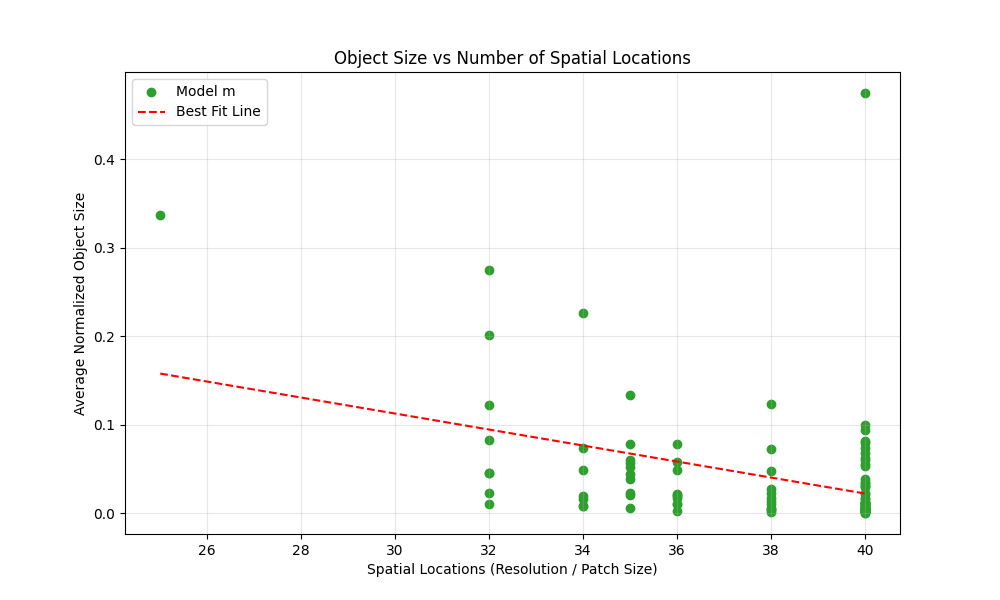
\includegraphics[width=0.48\linewidth]{figures/correlations/fixed_g1.png}
    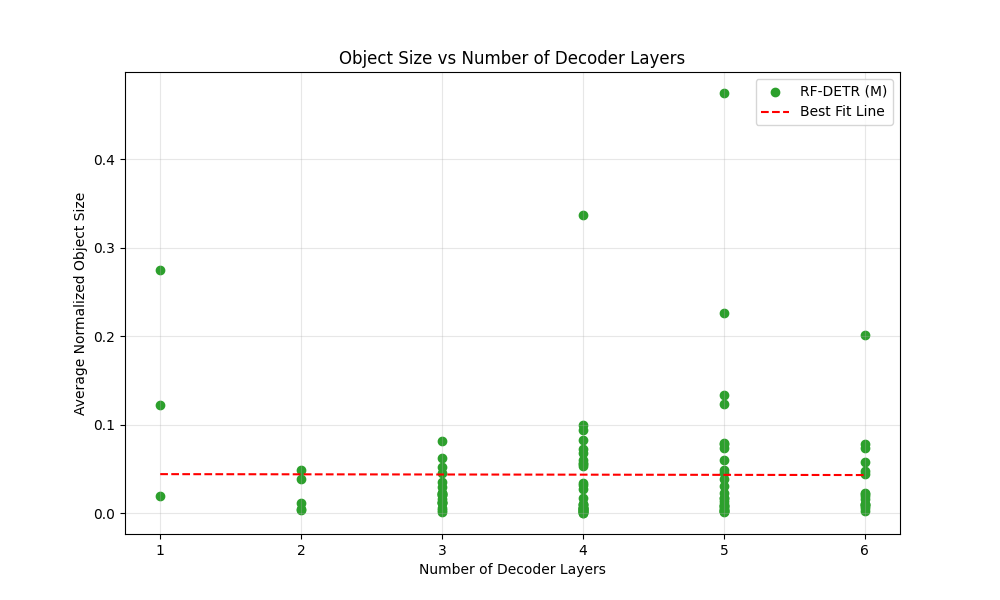
\includegraphics[width=0.48\linewidth]{figures/correlations/lr_size_dec_l.png}\\
    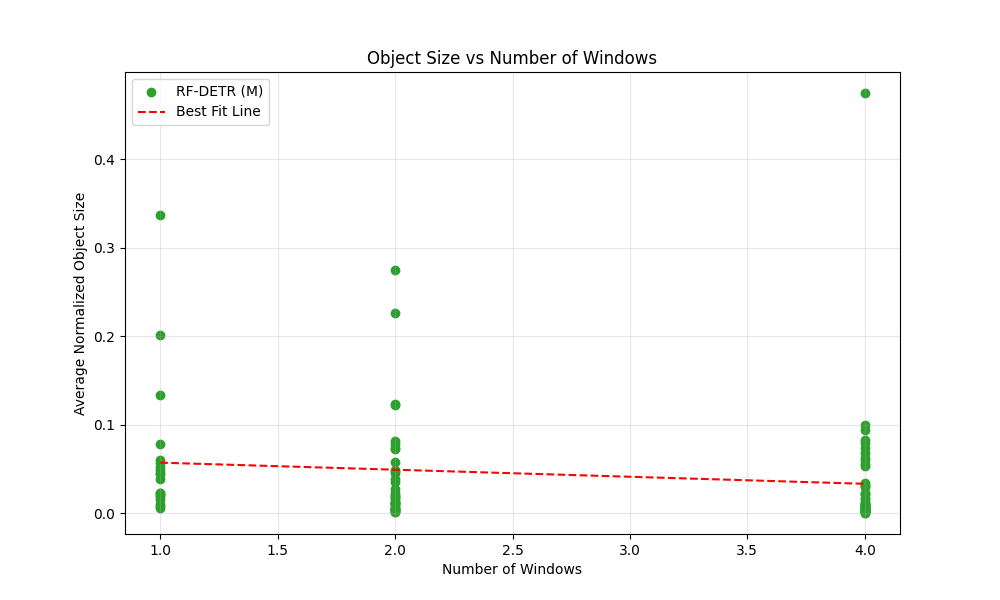
\includegraphics[width=0.48\linewidth]{figures/correlations/lr_size_win.png}
    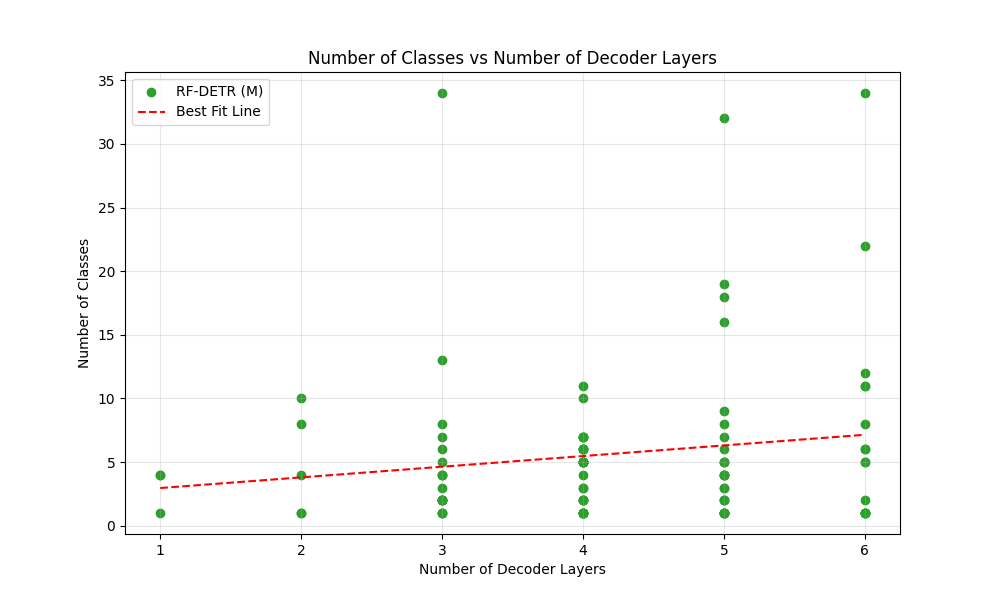
\includegraphics[width=0.48\linewidth]{figures/correlations/lr_numcl_decl.png} \\
     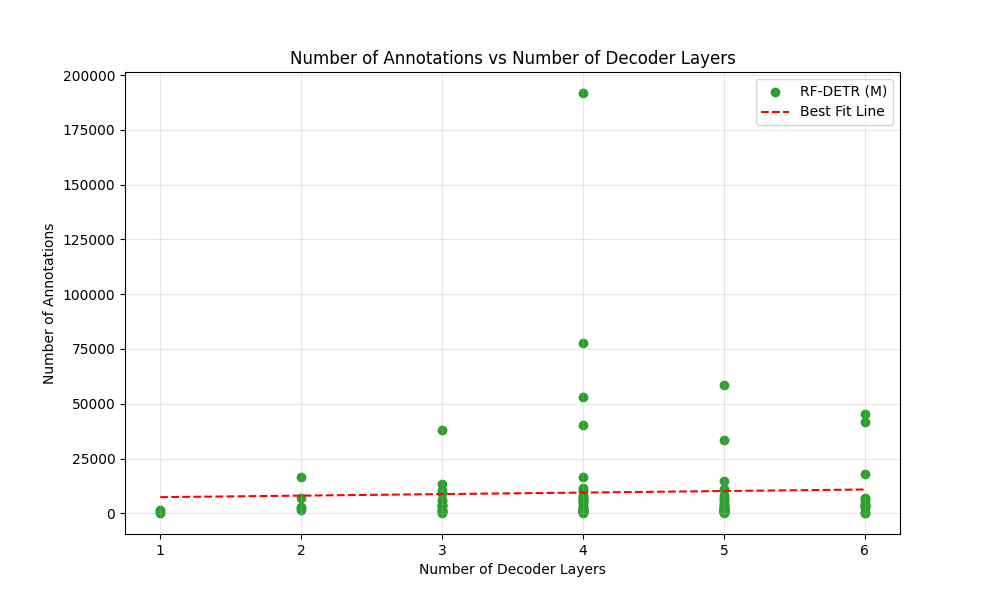
\includegraphics[width=0.48\linewidth]{figures/correlations/lr_annos_decl.png} 
    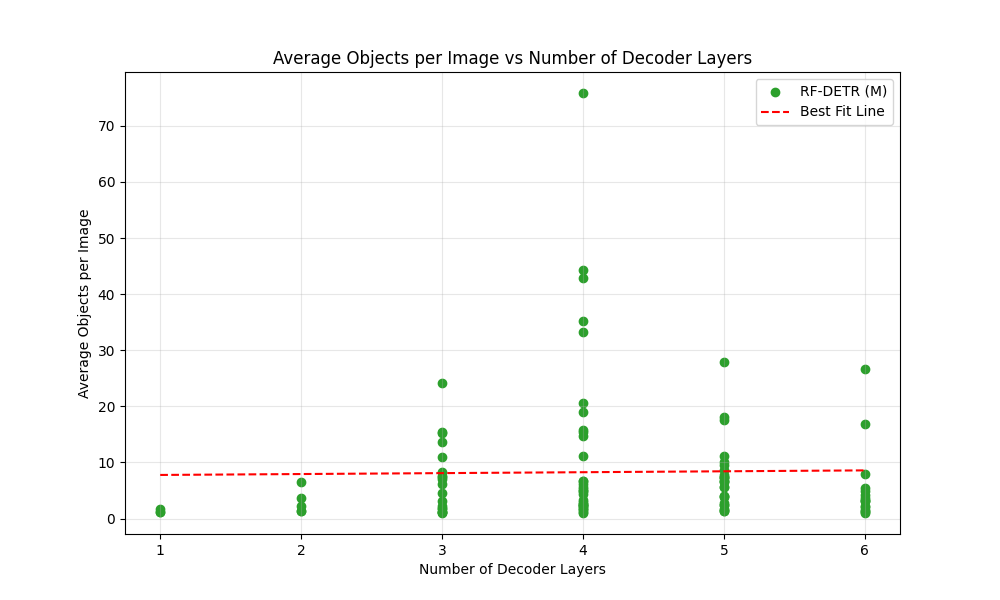
\includegraphics[width=0.48\linewidth]{figures/correlations/lr_obj_perim_decl.png} \\
    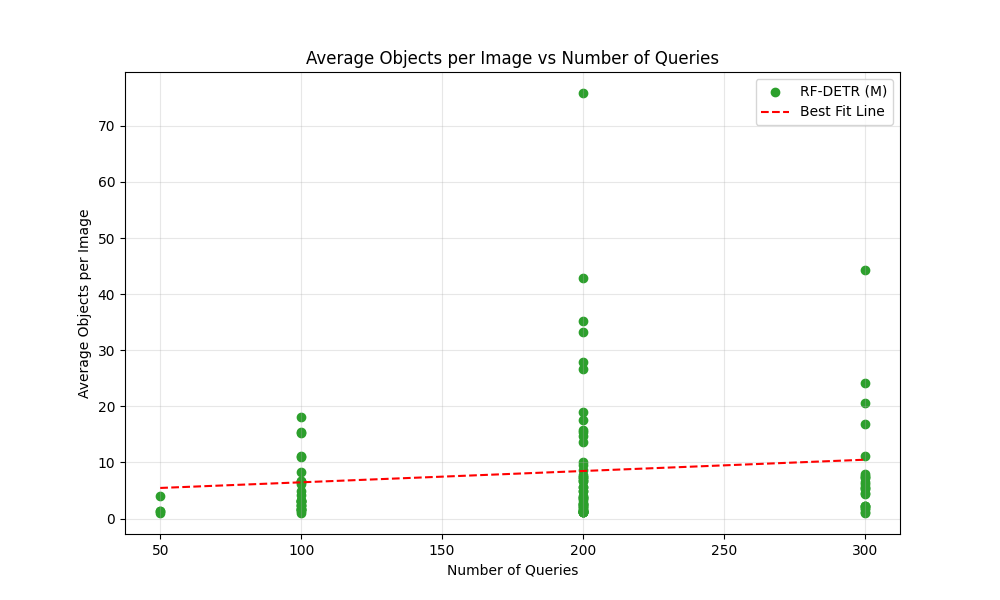
\includegraphics[width=0.48\linewidth]{figures/correlations/lr_avgobj_numq.png}
    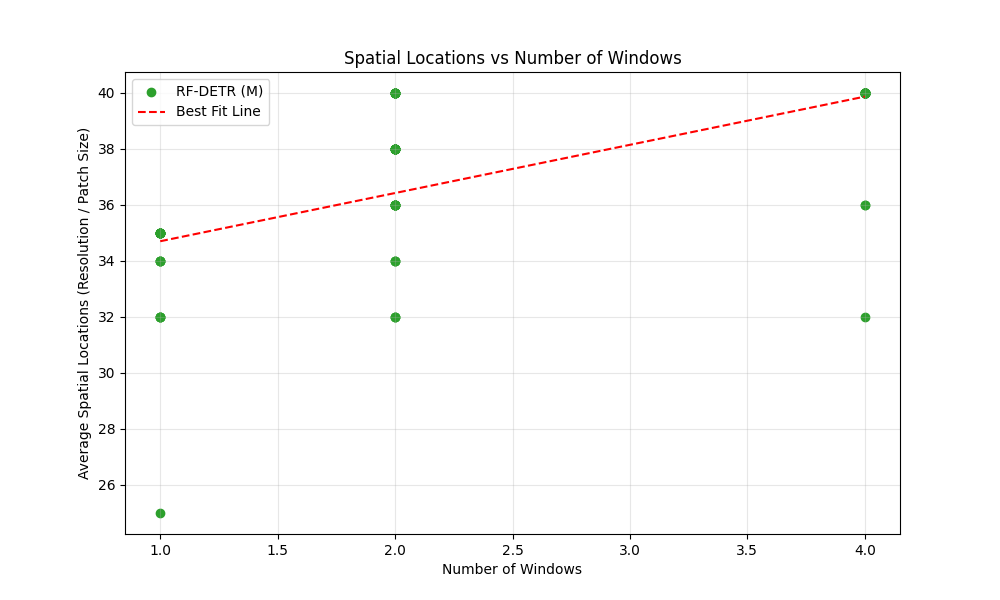
\includegraphics[width=0.48\linewidth]{figures/correlations/lr_splocs_numwin.png}
    \caption{\textbf{Impact of Dataset Characteristics on Tunable Knobs}. We visualize the correlation between key dataset characteristics and several tunable architectural knobs above. Across all subplots, individual points represent different datasets within RF100-VL while dashed lines show corresponding linear trends. Overall, the results indicate that object-centric properties of datasets such as average object size, number of classes, object density, and total annotations tend to have only modest influence on architectural choices like the number of decoder layers, number of windows, number of queries, and spatial resolution. Slight positive or negative trends appear in some cases (e.g., more classes or more objects per image loosely correlating with deeper decoders or higher query counts), but the scatter remains wide, suggesting no strong deterministic relationship. These findings highlight that while dataset characteristics offer some intuition for selecting model hyperparameters, optimal configurations ultimately depend on a combination of factors rather than any single dataset attribute.}
    \label{fig:dataset_char}
\end{figure}
{
\setlength{\tabcolsep}{0.25em}
\begin{table}[h]
\caption{\textbf{Regression Analysis.} We evaluate the linear relationships between various dataset characteristics and model parameters. Although these correlations are non-linear, the line-of-best-fit helps explain general trends. P-values indicate the significance of the correlation.} 
\label{tab:regression-results}
\scalebox{0.85}{
\begin{tabular}{|lccccc|}
\hline
\rowcolor{gray!10}
\textbf{Relationship} & \textbf{Slope} & \textbf{Intercept} & \textbf{R-squared} & \textbf{P-value} & \textbf{Std. Error} \\ \hline
\multicolumn{1}{|l|}{Average Object Size vs Number of Spatial Locations} & -0.009 & 0.384 & 0.148 & 0.000 & 0.002 \\ \hline
\multicolumn{1}{|l|}{Average Object Size vs Number of Decoder Layers} & -0.000 & 0.044 & 0.000 & 0.971 & 0.006 \\ \hline
\multicolumn{1}{|l|}{Average Object Size vs Number of Windows} & -0.008 & 0.065 & 0.019 & 0.170 & 0.006 \\ \hline
\multicolumn{1}{|l|}{Number of Classes vs Number of Decoder Layers} & 0.837 & 2.125 & 0.026 & 0.106 & 0.513 \\ \hline
\multicolumn{1}{|l|}{Number of Annotations vs Number of Decoder Layers} & 698.763 & 6654.795 & 0.001 & 0.706 & 1848.733 \\ \hline
\multicolumn{1}{|l|}{Average Objects per Image vs Number Decoder Layers} & 0.163 & 7.618 & 0.000 & 0.857 & 0.904 \\ \hline
\multicolumn{1}{|l|}{Average Objects per Image vs Number of Queries} & 0.020 & 4.457 & 0.019 & 0.171 & 0.015 \\ \hline
\multicolumn{1}{|l|}{Number of Spatial Locations vs Number of Windows} & 1.722 & 32.984 & 0.492 & 0.000 & 0.177 \\ \hline
\end{tabular}
}
\end{table}
}

\section{Impact of Fixed Architecture on RF100-VL}
We evaluate the impact of transferring a NAS architecture optimized for COCO to RF100-VL in Table \ref{tab:rf100-vl-fixed-arch} and Figure \ref{fig:fixed_arch_ablation}. We find that these fixed architecture models perform remarkably well without further dataset-specific NAS. Specifically, \method \ (large) model with a fixed architecture achieves the best performance among all prior real-time models on COCO. However, dataset-specific NAS yields  significant improvements. Notably, the performance delta from LW-DETR to the fixed architecture is comparable to the improvement from the fixed architecture to the NAS-optimized model on the target dataset for nano, small, and medium scale models.


\begin{figure}[h]
\centering
\begin{minipage}[c]{0.5\linewidth}
    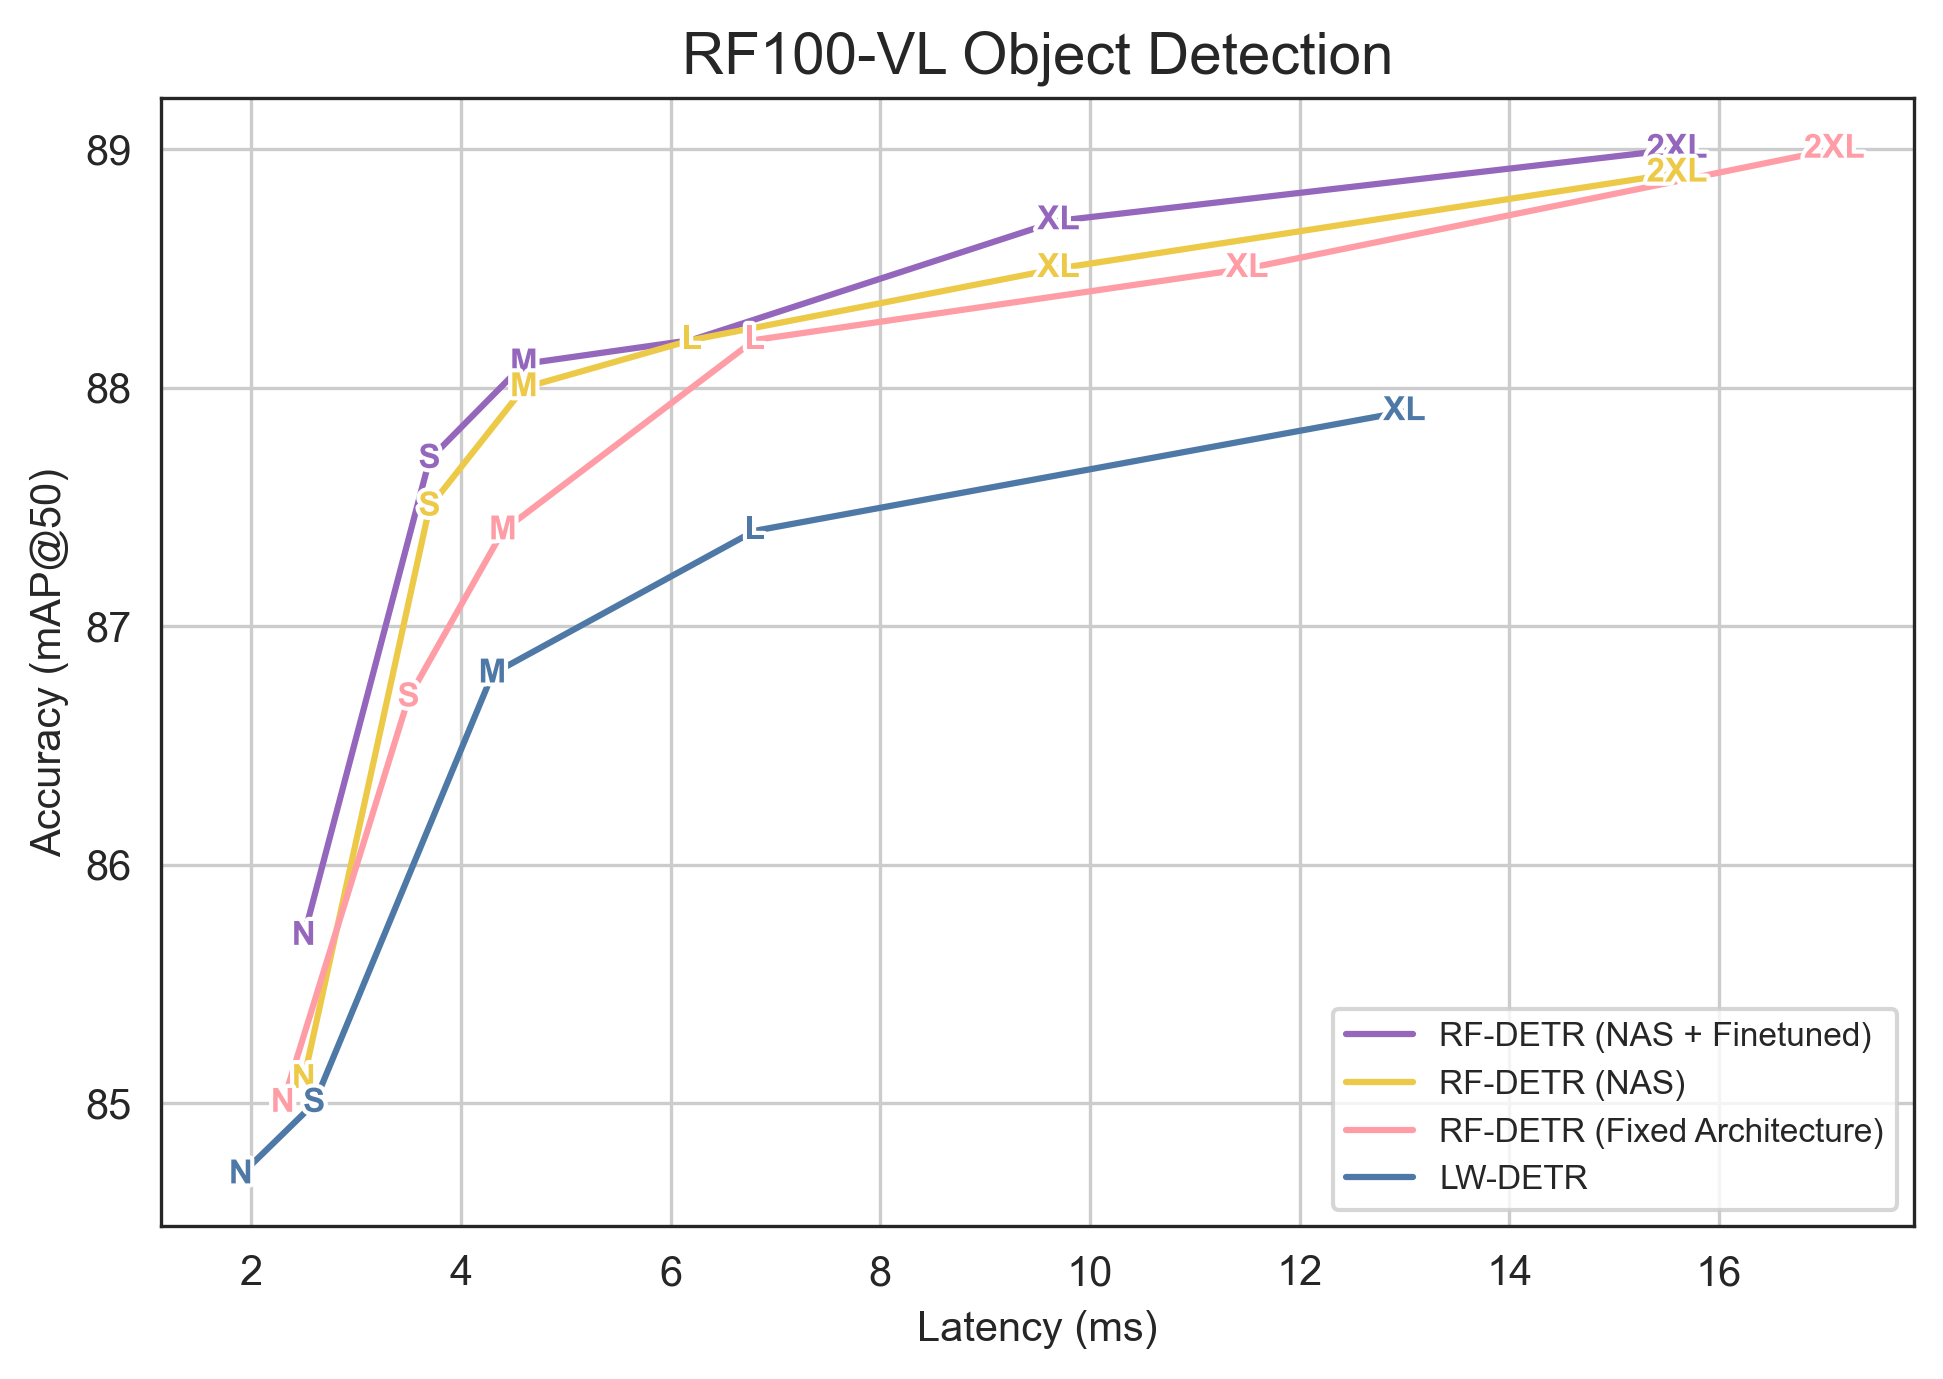
\includegraphics[width=\linewidth]{figures/latency_accuracy_RF100-VL_Object_Detection_mAPat50_NAS_search_ablation.png}
\end{minipage}\hfill
\begin{minipage}[c]{0.48\linewidth}
    \caption{{\bf Ablating Fixed Architecture RF100-VL}. We evaluate the benefit of dataset-specific NAS by transferring the COCO-optimized \method \ architecture to RF100-VL. Although the fixed architecture was not tuned for RF100-VL, it still outperforms LW-DETR. Running NAS directly on RF100-VL further improves performance over the fixed architecture. Additional fine-tuning provides consistent gains across all model sizes, with particularly strong improvements for smaller models. This is consistent with our observations on COCO object detection.}
    \label{fig:fixed_arch_ablation}
\end{minipage}
\end{figure}



{
\setlength{\tabcolsep}{0.25em}
\begin{table}[h]
\caption{\textbf{RF100-VL Fixed Architecture Evaluation.} We evaluate the transfer of architectures optimized for COCO to RF100-VL. Fixed architecture models perform well without additional dataset-specific NAS, with the \method \ (large) model achieving the best performance among prior real-time models. However, dataset-specific NAS provides significant further gains.} 
\label{tab:rf100-vl-fixed-arch}
\scalebox{0.7}{
\begin{tabular}{|lcccccccccc|}
\hline
\rowcolor{gray!10}
\textbf{Model} & \multicolumn{1}{c|}{\textbf{Size}} & \textbf{\# Params.} & \textbf{GFLOPS} & \multicolumn{1}{l|}{\textbf{Latency (ms)}} & \textbf{AP} & \textbf{AP$_{50}$} & \textbf{AP$_{75}$} & \textbf{AP$_S$} & \textbf{AP$_M$} & \textbf{AP$_L$} \\ \hline
\rowcolor{gray!10}
\multicolumn{11}{|l|}{\textbf{End-to-End Real-Time Object Detectors}}                                                                \\ \hline
\multicolumn{1}{|l|}{\method \ (Ours) Fixed Architecture}     & \multicolumn{1}{c|}{N}     &   30.5M    &   31.9      & \multicolumn{1}{c|}{2.3}             & 57.7   &   85.0   &  61.9    &   30.8  &   51.5  &   67.4  \\ \hline 
\multicolumn{1}{|l|}{\method \ (Ours)}     & \multicolumn{1}{c|}{N}     &   31.2M   &   34.5     & \multicolumn{1}{c|}{2.5}             & 57.8   &   85.1   &   62.5   &  30.1   &   52.2   &   67.2  \\ \hline
\multicolumn{1}{|l|}{\method \ w/ Fine-Tuning (Ours)}     & \multicolumn{1}{c|}{N}     &   31.2M   &   34.5     & \multicolumn{1}{c|}{2.5}             &  58.6  &  85.7   &   63.0  &  31.0  &  53.2   &  67.6  \\ \hline \hline
\multicolumn{1}{|l|}{\method \ (Ours) Fixed Architecture}     & \multicolumn{1}{c|}{S}     &   32.1M   &   59.8      & \multicolumn{1}{c|}{3.5}             & 60.2   &  86.7    &   65.0   &  34.2   &   54.4  &   68.9  \\ \hline 
\multicolumn{1}{|l|}{\method \ (Ours)}     & \multicolumn{1}{c|}{S}     &    33.5M   &    62.4    & \multicolumn{1}{c|}{3.7}             & 60.9   &   87.5   &   66.1   &  34.2   &   55.7  &  69.6   \\ \hline
\multicolumn{1}{|l|}{\method \ w/ Fine-Tuning (Ours)}     & \multicolumn{1}{c|}{S}     &    33.5M   &    62.4    & \multicolumn{1}{c|}{3.7}             &  61.2  &  87.7    &  66.1   &  34.9  &  55.6  & 69.5   \\ \hline \hline
\multicolumn{1}{|l|}{\method \ (Ours) Fixed Architecture}     & \multicolumn{1}{c|}{M}     &  33.7M     &   78.8    & \multicolumn{1}{c|}{4.4}             & 61.2   &   87.4   &  66.4    &   35.8  &   56.1  &   69.8   \\ \hline
\multicolumn{1}{|l|}{\method \ (Ours)}     & \multicolumn{1}{c|}{M}     &   33.6M    &   91.0     & \multicolumn{1}{c|}{4.6}             & 61.7   &    88.0  &   66.9   &  35.8   &   56.5  &   70.0  \\ \hline
\multicolumn{1}{|l|}{\method \ w/ Fine-Tuning (Ours)}     & \multicolumn{1}{c|}{M}     &   33.6M    &   91.0     & \multicolumn{1}{c|}{4.6}             & 62.0   &  88.1   &  67.1   &  36.2   &  56.4  &  70.2   \\ \hline \hline

\multicolumn{1}{|l|}{\method \ (Ours) w/ Fixed Architecture}     & \multicolumn{1}{c|}{L}     &   33.9M    &    125.6   & \multicolumn{1}{c|}{6.8}             & 62.2   &   88.2   &  67.8    &   37.7  &   57.0  &   70.5  \\ \hline
\multicolumn{1}{|l|}{\method \ (Ours)}     & \multicolumn{1}{c|}{L}     &   34.1M    &    119.1    & \multicolumn{1}{c|}{6.2}             &  62.0   &   88.1   &   67.3   &  36.9    &   57.1   &   70.2   \\ \hline
\multicolumn{1}{|l|}{\method \ (Ours) w/ Fine-Tuning}     & \multicolumn{1}{c|}{L}     &   34.1M    &    119.1     & \multicolumn{1}{c|}{6.2}             &  62.3   &   88.2   &   67.4   &   37.1   &   57.2   &  70.3    \\ \hline \hline
\multicolumn{1}{|l|}{\method \ (Ours, DINOv2-Base) w/ Fixed Architecture}     & \multicolumn{1}{c|}{XL}     &   126.4M    &    299.3       & \multicolumn{1}{c|}{11.5}             & 62.9   &  88.5    &   68.6   &  37.0   &   57.5  &   71.3  \\ \hline 
\multicolumn{1}{|l|}{\method \ (Ours)}     & \multicolumn{1}{c|}{XL}     &   35.0M    &    199.0    & \multicolumn{1}{c|}{9.7}             &   62.6   &  88.5   &  67.9   &   39.0   &   57.8   &  70.4  \\ \hline
\multicolumn{1}{|l|}{\method \ (Ours) w/ Fine-Tuning}     & \multicolumn{1}{c|}{XL}     &  35.0M    &    199.0      & \multicolumn{1}{c|}{9.7}             &   63.0  &   88.7   &   68.2   &   38.8   &   58.2   &   70.6   \\ \hline \hline
\multicolumn{1}{|l|}{\method \ (Ours, DINOv2-Base) w/ Fixed Architecture}     & \multicolumn{1}{c|}{2XL}     &   126.9M   &    438.4   & \multicolumn{1}{c|}{17.1}             & 63.2   &   89.0   &  69.3    &   38.4  &   58.4  &   71.5   \\ \hline
\multicolumn{1}{|l|}{\method \ (Ours, DINOv2-Base)}     & \multicolumn{1}{c|}{2XL}     &     123.5M    &    410.2    & \multicolumn{1}{c|}{15.6}             &  63.3   &   88.9   &    69.0  &  38.7    &   58.2   &   71.6   \\ \hline
\multicolumn{1}{|l|}{\method \ (Ours, DINOv2-Base) w/ Fine-Tuning}     & \multicolumn{1}{c|}{2XL}     &     123.5M    &    410.2     & \multicolumn{1}{c|}{15.6}             &   63.5  &   89.0   &   69.2   &   38.9   &   58.3   &   71.7   \\ \hline
\end{tabular}
}
%\raggedright\footnotesize
%$^{*}$ We use CUDA events to time pytorch models latencies for GDINO and LLMDet.
\end{table}
}
\section{Ablation on Backbone Architecture with RF20-VL}
In Table \ref{tab:backbone-rf20vl}, we reproduce our ablation on the impact of backbone architecture on downstream model performance (Table \ref{tab:backbone}) on RF20-VL. All trends from the main paper hold. 
{
\setlength{\tabcolsep}{0.6em}
\begin{table}[h]
\caption{\textbf{Ablation on Backbone RF20-VL.}} 
\label{tab:backbone-rf20vl}
\scalebox{0.7}{
\begin{tabular}{|lccccccccc|}
\hline
\rowcolor{gray!10}
\multicolumn{1}{|l|}{\textbf{LW-DETR (M) + Gentler Hyperparameters}} & \textbf{\# Params.} & \textbf{GFLOPS} & \multicolumn{1}{l|}{\textbf{Latency (ms)}} & \textbf{AP} & \textbf{AP$_{50}$} & \textbf{AP$_{75}$} & \textbf{AP$_S$} & \textbf{AP$_M$} & \textbf{AP$_L$} \\ \hline
\multicolumn{1}{|l|}{\quad w/ CAEv2 ViT/S-16-Truncated Backbone}     &  28.3M   & 83.7 &  \multicolumn{1}{c|}{4.3}             &  64.4  &  92.2    &   71.2   &  33.8   &  56.8   &  71.9   \\ \hline
\multicolumn{1}{|l|}{\quad w/ DINOv2 ViT/S-14 Backbone}     &      32.3M      &   78.2     &  \multicolumn{1}{c|}{4.6}             &  65.2  &  92.5    &   72.8   &  37.8   & 58.2    &  72.6  \\ \hline
\multicolumn{1}{|l|}{\quad w/ SigLIPv2 ViT/B-32 Backbone$^*$} & 105.1M     &     81.6   &  \multicolumn{1}{c|}{4.5}             & 62.2   & 91.0  & 67.8 & 28.9 & 54.1 & 70.3 \\ \hline
\multicolumn{1}{|l|}{\quad w/ SAM2 Hiera-S Backbone$^*$} & 44.0M &  109.1 &  \multicolumn{1}{c|}{11.2}   &  65.2  &  92.5  & 72.7  & 37.8  & 58.2  &  72.1  \\ \hline
\end{tabular}
}
\end{table}
}

\section{Analysis on Buffering}
\label{appendix:throtting}

We further analyze the impact of buffering on the relative ordering of inference speed in Table \ref{tab:buffering}. Notably, we find that buffering beyond 200ms does not change latency measurements. However, we acknowledge that adding a 200ms buffer after every forward pass considerably increases overall inference time. Future work should consider alternatives to buffering to address power throttling.


{
\setlength{\tabcolsep}{2.6em}
\begin{table}[h]
\centering
\caption{\textbf{Analysis on Buffering.} We evaluate models with different amounts of buffering between consecutive forward passes. We find that buffering beyond 200ms does not provide any additional stability to latency measurements.}
\label{tab:buffering}
\scalebox{0.7}{
\begin{tabular}{|l|c|c|c|c|c|}
\hline
\rowcolor{gray!10}
\textbf{Model} & \textbf{mAP} & \textbf{0 ms} & \textbf{200 ms} & \textbf{400 ms} & \textbf{800 ms} \\
\hline
YOLOv8 (M)     & 47.3 & 5.5 ms & 5.4 ms & 5.4 ms & 5.4 ms\\ \hline
YOLOv11 (M)    & 48.4 & 5.0 ms & 5.0 ms & 5.1 ms & 5.1 ms\\ \hline
RT-DETR (R18)  & 49.0 & 4.4 ms & 4.4 ms & 4.4 ms & 4.4 ms\\ \hline
LW-DETR (M)    & 52.6 & 4.5 ms & 4.3 ms & 4.3 ms & 4.3 ms\\ \hline
D-FINE (M)     & 54.9 & 5.7 ms & 5.4 ms & 5.4 ms & 5.4 ms \\ \hline
RF-DETR (M)    & 54.7 & 4.7 ms & 4.4 ms & 4.4 ms & 4.4 ms\\
\hline
\end{tabular}
}
\end{table}
}

\section{Discussion on Notable Discovered Architectures}
\label{appendix:trends}
% points to hit: 
% - more extremal architectures seem to benefit more from further finetuning
% - seg has the same head for all sizes, just varying resolution
% - patch size / resolution doesn't matter for RF-DETR, just number of spatial locations
% - still, prefers to use more 'central' values .. 
% - DOES matter for seg, since effectively controls the bilinear upsample ratio
% - see seg models preferring smaller kernels -> as if a smaller upsample ratio if pretending fixed image size
% - surprisingly, seg models prefer 200 queries .. better accuracy than the 300 version
% - windows 2 seems to be generally best, interesting because class token structure ie 4 has tradeoff where there are more duplicated class tokens
% - models tend to jointly scale number of positional encodings and number of decoder layers .. a set of optimal configs (controlling for queries) is [insert original N S and M here]
% - optimal families tend to be generated by holding some factor constant and scaling others .. see seg and original N S and M .. similar to the 'compound scaling' of efficientnet
% - 0 dec layers is often optimal for very fast models
% - RF100-VL models tend to use fewer decoder layers and prefer more spatial locations
% - sometimes the 'best' model will still be fairly fast

% Several trends emerge from our weight-sharing NAS. First, we note that \method \ models optimized for COCO exhibit predictable compound scaling \citep{tan2019efficientnet}: patch size, number of queries and number of windows remain fixed, while resolution and decoder depth increase. Specifically, the Pareto-optimal family maintains a patch size of $16$, $300$ queries, and $2$ windows, while scaling resolution and decoder layers. \method \ (nano) uses a resolution of $384$ with 2 decoder layers, \method \ (small) uses a resolution of $512$ with 3 decoder layers, and \method \ (medium) uses a resolution of $576$ with 4 decoder layers. \method-Seg models follow a similar pattern between model sizes, fixing queries ($200$), decoder layers ($4$), patch size ($12$), and windows ($2$), while only scaling resolution. Specifically, \method-Seg (nano) uses a resolution of $312$, \method-Seg (small) uses a resolution of $384$, and \method-Seg (medium) uses a resolution of $432$. Interestingly, \method-Seg models using $200$ queries outperform models using $300$ queries.

Several trends emerge from our weight-sharing NAS. First, we note that all tunable ``knobs'' are used when defining Pareto-optimal model families, validating our search space. This suggests that expanding the search space may further improve downstream performance.

Across Pareto-optimal models, patch size is consistent within model families. For example, the optimal patch size for RF-DETRs \ with a DINOv2-S backbone is 16, RF-DETRs \ with a DINOv2-B backbone is 20, and \method-Segs with a DINOv2-S backbone is 12. Pareto-optimal models also jointly scale encoder and decoder compute: patch size, number of windows, and resolution impact the encoder, while decoder depth, and number of queries affect the decoder. For \method-Seg, scaling resolution impacts the segmentation head. We find that using 2 windows in the encoder is typically optimal and resolution scales within a model family as we increase latency. On COCO, \method \ scales decoder depth while keeping the number of queries fixed, while \method-Seg simultaneously scales both axes. This likely reflects a minimum viable segmentation head depth; to offset its latency, \method-Seg reduces its total number of queries, yielding a thin, deep decoder, in contrast to \method’s wide, shallow decoder.

%For the decoder, on COCO the detector model keeps queries constant and scales decoder layers only, while for the segmentation model both are scaled simultaneously. This may be because the depth of the segmentation head is tied to the number of decoder layers, and there may be a certain minimum number of layers in the segmentation head that produce viable masks, so even the lowest latency model uses at least that number of layers. To compensate for the additional latency of those decoder layers, the segmentation model trades off the number of queries it uses to get lower latency for smaller model sizes, which effectively reduces the width of the decoder. While the object detector evaluated on COCO prefers a wide and shallow decoder, the segmentation model prefers a thin and deep decoder. 

Next, we find that \method's performance is more correlated with the total number of spatial locations (e.g. resolution divided by patch size) rather than resolution or patch size alone. Scaling resolution with a fixed patch size yields similar results to scaling patch size with a fixed resolution, since vision transformers are agnostic to absolute input resolution after the patchify-and-project operation. To verify this, we constructed an alternative model family with fixed resolution ($640$) and varied patch sizes to preserve the total number of spatial locations. Specifically, we evaluate \method \ (nano) with a patch size of $27$, \method \ (small) with a patch size of $21$, and \method \ (medium) with a patch size of $18$. Surprisingly, all model results are nearly identical to the Pareto-optimal family. Notably, patch sizes of $27$ and $18$ were unseen during training, demonstrating \method's strong generalization to novel patch sizes \citep{beyer2023flexivit}. However, we find that this trend does not hold for \method-Seg because segmentation features are always upsampled to $\frac{1}{4}$ of the input image resolution. As a result, scaling \method-Seg's input resolution affects both the number of spatial locations and the segmentation feature resolution. Specifically, \method-Seg (nano, small, medium) uses input resolutions of 312, 384, and 432 with patch size 12, yielding segmentation feature resolutions of 78, 96, and 108 and 26, 32, and 36 spatial locations, respectively. In contrast, increasing patch size alone (e.g., patch size 16 at input resolution 576) preserves spatial locations while increasing segmentation feature resolution. As a result, although \method\ (medium) and \method-Seg (medium) both use 36 spatial locations, \method-Seg operates at lower input resolution, demonstrating that coupling segmentation feature resolution with input resolution shifts the Pareto-optimal operating point.

Further, we find that most Pareto-optimal \method \ models perform best with 2 windows, whereas LW-DETR achieves the best performance with 4 windows. We attribute this difference to how each architecture handles class tokens. LW-DETR’s CAEv2 backbone omits the class token, while \method's DINOv2 backbone relies on it as a key part of pre-training. To make windowed attention compatible with class tokens, we duplicate the class token for each window. During global attention, window-level class tokens attend to one another, while all other tokens attend to all class tokens. In practice, \method \ (nano), \method \ (small), and \method \ (medium) all use 2 windows, since duplicating class tokens for additional windows reduces runtime efficiency. As a result, unlike LW-DETR, \method \ does not benefit from scaling to 4 windows.

%To generate our model based on DINOv2-B, we follow the scaling strategy from ViT-S to ViT-B and just double the width of all layers in the model. We find that this is sufficient to gain strong and differentiated performance when we allow NAS to explore the axis of variation we've defined. Notably, different from LW-DETR's larger variants, we don't use higher resolution feature maps from the backbone.

Lastly, we note that dataset characteristics influence optimal discovered architectures. We find that the optimal low latency models on RF100-VL tend to use fewer queries than the COCO models of equivalent latency. We attribute this to RF100-VL datasets having fewer objects per image than COCO.


% new points to hit:
% - all axis are used
% - single model families like to use a single patch size
% - seg prefers fewer queries because it requires more layers in the seg head
% - finetuning doesn't help much on COCO except for nano. likely due to acting as regularizer. helps on rf100vl likely because the 100 epochs is not enough time for the model to converge
% - dinov2-b backbone variant just doubles the width of the network and that's sufficient for good results



\section{Visualizing Model Predictions}
We visualize model predictions from \method \ (nano) and relevant detection and segmentation baselines in Figure \ref{fig:visuals}. We find that \method \ (nano) predicts fewer false positives (e.g. mistaking {\tt sign post} for {\tt person}). Similarly, \method-Seg. (nano) predicts more precise object boundaries.

\begin{figure}[h]
    \centering
    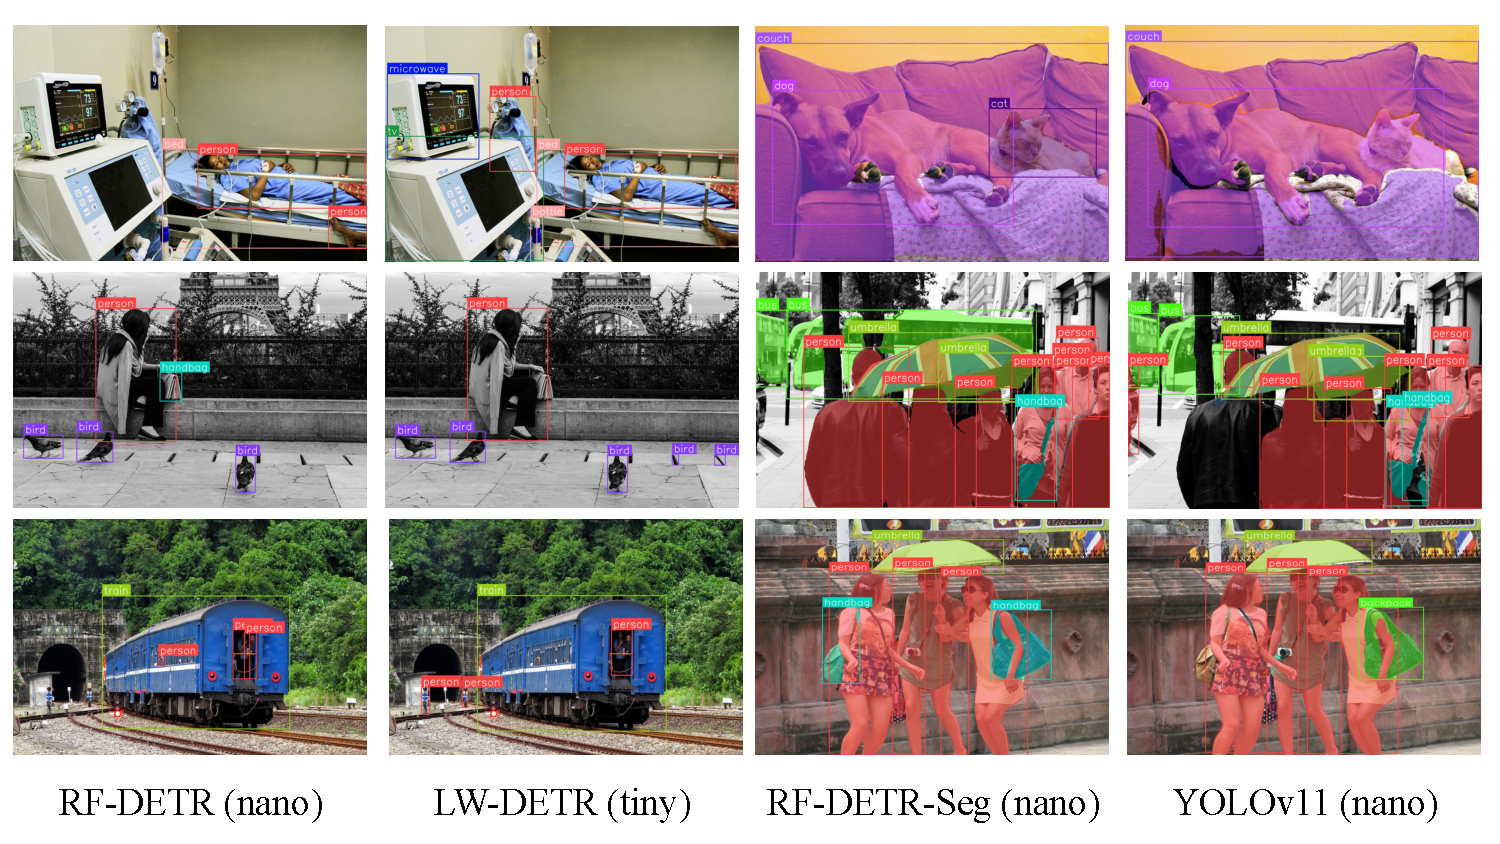
\includegraphics[width=0.9\linewidth]{figures/visuals.pdf}
    \caption{{\bf Visualizing Model Predictions}. On the left, we compare detections from \method \ (nano) and LW-DETR (tiny). On the right, we compare instance segmentation masks from \method-Seg (nano)  and YOLOv11 (nano)}
    \label{fig:visuals}
\end{figure}







